\documentclass[a4paper,11pt]{report}
\usepackage[T1]{fontenc}
\usepackage[utf8]{inputenc}
%\usepackage{lmodern}
\usepackage{baskervald}
\usepackage{hyperref}
\usepackage{graphicx}
\usepackage[finnish]{babel}
\usepackage{caption}
\usepackage{gensymb}
\captionsetup{labelformat=empty}
\usepackage{wrapfig}
\usepackage{tikzpagenodes}
\usepackage{multicol}

\begin{document}


\begin{titlepage}
	\centering
	{\scshape\Huge Oluesta \par}
	\vspace{5cm}
	
\includegraphics[width=0.3\textwidth]{mugbeer}\par\vspace{1cm}

	{\scshape\Large Perustietoa oluesta ja oluenvalmistuksesta\par}

	\vfill
	
	{\large Polyteknikkojen olutkulttuurin edistämisyhdistys POLKU ry \\ Espoo 2015}
\end{titlepage}
\newpage\null\thispagestyle{empty}

\tableofcontents

\chapter{Pari sanaa järjestävästä seurasta}

%\vspace{-2.5cm}
%\begin{figure}[ht]
%\centerline{
%
\includegraphics[width=10cm]{polkulogo.png}
%}
%\end{figure}

\begin{tikzpicture}[remember picture,overlay]
\node[anchor=east,inner sep=0pt] at (current page text area.east|-0,7cm) {
\includegraphics[height=7cm]{polkulogo}};
\end{tikzpicture}

Olut on erottamaton osa teekkarikulttuuria. 1990-luvun alussa Suomessa alkoi nousta yleinen kiinnostus olutkulttuuria kohtaan. Ensimmäisten olutseurojen joukossa, jo vuonna 1991, perustettiin otaniemeläistä olutkulttuuria ylläpitämään ja kehittämään Polyteknikkojen olutkulttuurin edistämisyhdistys POLKU. 

Perinteisten kilta- ja yhdistystapahtumien suhde olueen on usein kvantitiivinen. Lasiin sylkemättä ja pikkurilliä pystyyn nostamatta POLKU pyrkii toiminnassaan korostamaan oluen nauttimisen laadullista puolia: oluen maailma on makujen ja nautinnon maailma. POLKUn toiminnan muotoja ovat muun muassa ekskursiot olutmaihin ja -kohteisiin, maistelut ja saunaillat. Olut maistuu parhaalta oikeanlaisesta tuopista, oikeassa lämpötilassa tarjoiltuna rauhallisesti nautiskeltuna, tietenkään hyvää seuraa unohtamatta!

POLKU tukee myös kotioluen valmistusharrastusta teekkareiden keskuudessa. Panokursseja on järjestetty jo vuosia ja ne ovat aina olleet hyvin suosittuja. Varsinkin aloitelevalle harrastajalle merkittävää on, että POLKU tarjoaa panimotilan ja -laitteistoa jäsenistönsä käytettäväksi

Tervetuloa olutkurssille ja mukaan POLKUn toimintaan!

\subsection*{Toimitus}

\subsubsection*{Ensimmäinen painos}

Polkun esittely - Jukka Lehtniemi, Oluen historia - Kari Koskinen, Oluttyylit - Henrik Kettunen. Oluen maistaminen ja juominen - Eero Rinne, Oluen valmistuksen teoria - Jaakko Ala-Paavola. Kotioluen valmistus - Mikko Sojonen. Taitto jo muu toimitus: Vexi Savijoki

\subsubsection*{Toinen painos}

Eero Rinne ja Vexi Savijoki

\subsubsection*{Kolmas painos}

Panu Lahtinen (konvertointi LaTeX -muotoon)

\subsubsection*{Neljäs painos}

Juha Västi

\chapter{Oluen historia}

\begin{tikzpicture}[remember picture,overlay]
\node[anchor=east,inner sep=0pt] at (current page text area.east|-0,5cm) {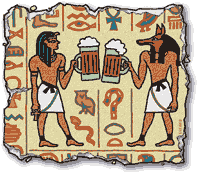
\includegraphics[height=4cm]{hieroglyph.png}};
\end{tikzpicture}


\section{Muinaishistoria}

Jos puhutaan ihmiskunnan kirjoitetusta historiasta, voidaan sanoa, että olutta on tehty ''aina''. Ensimmäiset olueksi luokiteltavat tuotteet on tehty paljon ennen kirjoitustaidon keksimistä. Tämän vuoksi oluelle ei voidakaan määritellä tarkkaa syntymähetkeä. Selvää on kuitenkin se, että olut ei ole mikään vahingossa keksitty tuote vaan sen valmistusta on tarkoituksellisesti kehitelty kaikkialla maailmassa.

Useimmiten oluen historian katsotaan alkaneen Sumerista, Kaksoisvirranmaasta, missä noin 6000 vuotta vanhoissa savitauluissa kerrotaan viljasta valmistetusta käyneestä juomasta, Sikarusta. Sumerin alueen naisväestö leipoi ohraleipiä, jotka laitettiin veteen käymään. On arvioitu, että Sumerin alueen viljatuotannosta peräti 40\% käytettiin oluen tuotantoon.

Parissa tuhannessa vuodessa olut oli jo vakiinnuttanut asemansa osana sumerien yhteiskuntaa. Tästä osoituksena on esimerkiksi Hammurabin lakien 108. artikla: ''Jos kapakoitsijatar ei ota vastaan viljaa juovutusjuoman hintana, vaan ottaa hopeaa suuren kivipunnuksen mukaan tai saatua juovutusjuoman arvon pienemmäksi kuin viljan arvon, niin ko. kapakoitsijatar todistettakoon vikapääksi ja heitettäköön veteen''.

Kaksoisvirranmaasta olut levisi valloitusten myötä kaikkialle lähialueille ja nykyäänkin heprean kielen sana ''shekar'', joka tarkoittaa ''olla päihtynyt'' tai ''päihtymys'' on eittämättä babylonialaista alkuperää. Kaksoisvirranmaasta oluen valmistus levisi myös Egyptiin, jossa sitä käytettiin aluksi uskonnollisissa riiteissä, mutta myöhemmin laajemminkin tervetuliaisjuomana, vaihtorahana ja palkkoina.

Kuitenkaan ei voida ajatella oluen syntyneen Keski-idässä, josta se sitten olisi levinnyt muualle maailmaan. Todellisuudessa olutta on tehty, ainakin jossain muodossa, kaikilla mantereilla joilla kehittyneet sivilisaatiot ovat nähneet päivänvalon. Eurooppalainen kulttuuri-imperialismi on nyttemmin levittänyt nykyisenkaltaisen oluen ympäri maailman, mutta tämä ei tarkoita sitä, etteikö muissakin maailman kulttuureissa olisi olutta tunnettu.

Kun babylonialaiset ja egyptiläiset vielä 2000--3000 vuotta ennen ajanlaskumme alkua valmistivat oluensa arkaaisella olutleipä-menetelmällä, olivat kiinalaiset siirtyneet jo varhaisteollisiin valmistusmenetelmiin. Voidaankin perustellusti sanoa, että nykyisenkaltainen oluenvalmistusmenetelmä on keksitty ensimmäisenä Kiinassa. Kiinassa valmistettiin tuolloin oluita lähinnä hirssistä, vehnästä ja riisistä suurin piirtein vastaavin mäskäysmenetelmin kuin nykyäänkin.

Oluen raaka-aineena käytettiin kullakin alueella tyypillisesti kasvavaa viljaa: Amerikoissa pääraaka-aine oli yleensä alueella viljelty maissi tai maniokki, Afrikassa käytettiin hirssiä ja durraa. Kiinassa ja Kaakkois-Aasiassa hirssi ja ohra lopulta väistyivät riisin tieltä oluen raaka-aineena.

\section{Eurooppalainen olut}

Kun Keski-idässä olut sai lopulta väistyä viininvalmistuksen tieltä, säilytti se kuitenkin vahvan asemansa pohjoiseurooppalaisten kansojen juomana. Olut ja viini kilpailivat Euroopassa pitkään valta-asemasta ja ''kristillinen'' viini sai lopulta voiton Etelä-Euroopassa, oluen jäädessä pohjoisempien kansojen juomaksi. Jo vuoden 1000 paikkeilla Viini-Euroopan ja Olut-Euroopan raja oli suurin piirtein niillä kohdin, missä se nykyisinkin on, eli Etelä-Saksan ja Pohjois-Ranskan alueella.

Vuoden 1000 tienoilla teollinen oluentuotanto keskittyi lähinnä majataloihin ja munkkiluostareihin. jotka vähitellen korvasivat kotona valmistetun oluen kaikkialla Euroopassa. Vanha kotona tehdyn oluen traditio on tosin vielä Suomessa nähtävissä omassa primitiivioluessamme eli sahdissa.
\begin{wrapfigure}{r}{0.55\textwidth}
  \begin{center}
    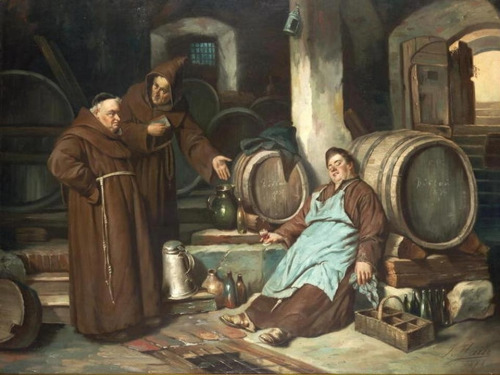
\includegraphics[width=0.53\textwidth]{drunkmonk}
    \caption{Giuseppe Marastoni: Humaltunut munkki}
  \end{center}
  \end{wrapfigure}

Olut oli tuohon aikaan hyvin paikallinen tuote. Jokaisella kylällä ja suuremmalla maatilalla oli omaa oluen tuotantoa. Tällainen paikallisoluiden traditio on edelleen voimissaan esimerkiksi Saksassa, jossa suuret maailmanlaajuiset merkit eivät ole onnistuneet tuhoamaan moninaisia paikallisia erikoisuuksia.

1400-luvulla humalasta tuli yleisin oluen mauste, ja olut alkoi muutenkin muistuttaa hyvin paljon nykyisia pintahiivaoluita. Mainittakoon vielä, että vuonna 1516 Baijerin herttuat säätivät niin sanotun Reinheitsgebot-lain, joka määräsi oluen ainoiksi sallituiksi valmistusaineiksi ohran, humalan ja veden. Hiivaahan ei tuolloin vielä tunnettu, vaan valmistus perustui villihiivojen aiheuttamaan käymiseen.

Seuraava mullistus oluenvalmistuksessa oli teollinen vallankumous, joka sai alkunsa Englannissa 1700-luvulla. Rautatieverkoston rakentaminen tarjosi panimoille mahdollisuuden laajamittaiseen kaupankäyntiin ja laajensi oluen markkinoita. Tämä mahdollisti myös entistä suurempien ja tehokkaampien panimoiden synnyttämisen.

\section{Lager-oluen synty}

Samaan aikaan kun teollinen vallankumous 1800-luvulla synnytti yhä suurempia panimoita, mullisti markkinoita uusi valmistustekninen innovaatio: pohjahiiva. Oluenvalmistajat olivat pitkään tienneet, että mikäli olut pidettiin matalassa lämpötilassa, se ei pilaannu niin helposti. Lisäksi huolellisella jäähdyttämisellä saadaan käymisen aikana muodostuva hiiva painumaan säiliöiden pohjalle, ja oluesta tulee kirkasta.

Tälle ilmiölle keksi tanskalainen Hansen vuonna 1883 selityksen ja totesi, että on mahdollista eristää erityisiä hiivalaatuja, jotka käyvät nimenomaan alhaisissa lämpötiloissa ja tuottavat tasalaatuisia, hyvin säilyviä oluita. Syntyi Lager-olut. Lager-sanahan tarkoittaa saksaksi varastoa ja viittaa siten nimenomaan kyseisen oluen hyvään säilyvyyteen. Tämän innovaation mahdollisti Louis Pasteurin kehittämä mikrobiologia, jonka myötä hiivan toiminta ymmärrettiin osaksi oluen ja esimerkiksi juustojen valmistusta.

Uusi tekniikka vaati huomattavia investointeja, mikä pakotti monet pienpanimot lopettamaan toimintansa tai liittoutumaan toisten panimoiden kanssa. Erilaisten alueellisten oluiden määrä laski merkittävästi samaan aikaan, kun hyvin säilyvä ja helposti juotava olut valtasi yhä uusia markkina-alueita. Jopa perinteisissä viinimaissa olut alkoi saavuttaa yhä kasvavampaa suosiota.

150 vuoden aikana 12 vuosisataa suhteellisen muuttumattomana säilynyt panimoperinne koki täydellisen muutoksen ja viimeisen sadan vuoden aikana panimojen lukumäärä onkin laskenut merkittävästi ja erilaiset paikalliset erikoisuudet ovat korvautuneet tyypillisillä Lager-oluilla. Näiden oluiden pääraaka-aine on ohra, vaikka muitakin raaka-aineita (lähinnä vehnää, maissia, riisiä ja ruista) käytetään.

Olut on nykyään suositumpaa kuin koskaan aiemmin, mutta valmistus on samaan aikaan keskittynyt yhä suurempien tuottajien käsiin. Viime aikoina tilanne on olutharrastajan näkökulmasta tosin parantunut. Monien oluenharrastajien suosiessa pienempien panimoiden tuottamia maukkaampia oluita on ympäri maailmaa syntynyt suuri määrä pienpanimoita, jotka tuottavat erikoisoluita vaativalle asiakaskunnalle. Tämä ei toki muuta sitä tosiasiaa, että 90\% maailman oluesta on nykyään tavanomaista ''peruslageria''.

\section{Olut Suomessa}

Suomi on perinteinen olutmaa. Pohjoinen sijainti ei mahdollista viinien suurimittaista tuotantoa, vaan ainoa alueelle ''luontaisesti'' sopiva alkoholijuoma on olut. Osoituksena pitkästä historiassa on esimerkiksi Kalevala, jossa oluen syntyä kuvataan pidemmälti kuin, sinänsä paljon vähäpätöisemmän asian, maailman syntyä.

Suomessa oluita tehtiin tyypillisesti kaikissa suuremmissa maataloissa ja Suomi maksoi osan Ruotsin kruunulle kannetuista veroistaankin oluella. Oluenvalmistuksen perinteet ovat yhä nähtävissä perinteisessä sahdin valmistuksessa. Myös teollisessa tuotannossa Suomi on ollut jonkinasteinen edelläkävijä: Nikolai Sinebrychoff perusti Helsinkiin Pohjoismaiden ensimmäisen panimon jo vuonna 1819.

Olutkulttuurin alasajo Suomessa toteutettiin 1.6.1919 voimaan tulleen kieltolain avulla. Perinteisestä oluen valmistuksesta ja nauttimisesta tehtiin ''kansan raitistamisen'' nimissä laitonta. Laki epäonnistui tavoitteessaan, sillä sivistynyt oluen nauttiminen muuttui pirtusalakuljetuksen myötä väkevien, kirkkaiden viinojen juomiseksi -- Suomesta tuli ''vodkamaa''.

Kieltolaki kumottiin vuonna 1932, mutta katkaistu oluen valmistuksen perinne ei päässyt elpymään. Nyt oluen valmistusta ja myyntiä valvoi valtion alkoholimonopoli. Lainsäädännöllisin keinoin erilaisten olut-tyyppien valmistusta rajoitettiin ja panimoiden oli pakko keskittyä ainoastaan muutamaan merkkiin, minkä vuoksi saatavilla oli lähinnä tavanomaisia lagereita.

Alkoholilainsäädäntö on EU-Suomessa vapautumassa, jonka seurauksena maahan on viimeisen reilun kymmenen vuoden ajan syntynyt runsaasti uusia pienpanimoita, jotka jatkavat osaltaan oluenvalmistuksen vanhoja perinteitä. Myös suuremmat panimot ovat huomaamassa, että oluita juova kansa haluaa muutakin kuin tavallista lageria. Kirjoitushetkellä uusia pienpanimoita tuntuu Suomeen syntyvän kuin sieniä sateella, ja voikin oikeutetusti sanoa, että Suomen olutkulttuuri on elinvoimaisempi kuin koskaan ennen.


\section*{Lähteet}

\begin{itemize}
\item{Christian Berger ja Philippe Dupoe-Laurence, Oluen ystävän opas, Otava}
\item{Aino Forsius, Viinasta, oluesta ja raittiustyöstä Hollolassa ja Lahden kauppalassa, \url{http://www.saunalahti.fi/arnoldus/alkorait.html}}
%\item{\url{http://pubs.acs.org/subscribe/archive/tcaw/10/i12/html/12chemchron.html}}
\end{itemize}



\chapter{Oluttyylit}

\begin{tikzpicture}[remember picture,overlay]
\node[anchor=east,inner sep=0pt] at (current page text area.east|-0,5cm) {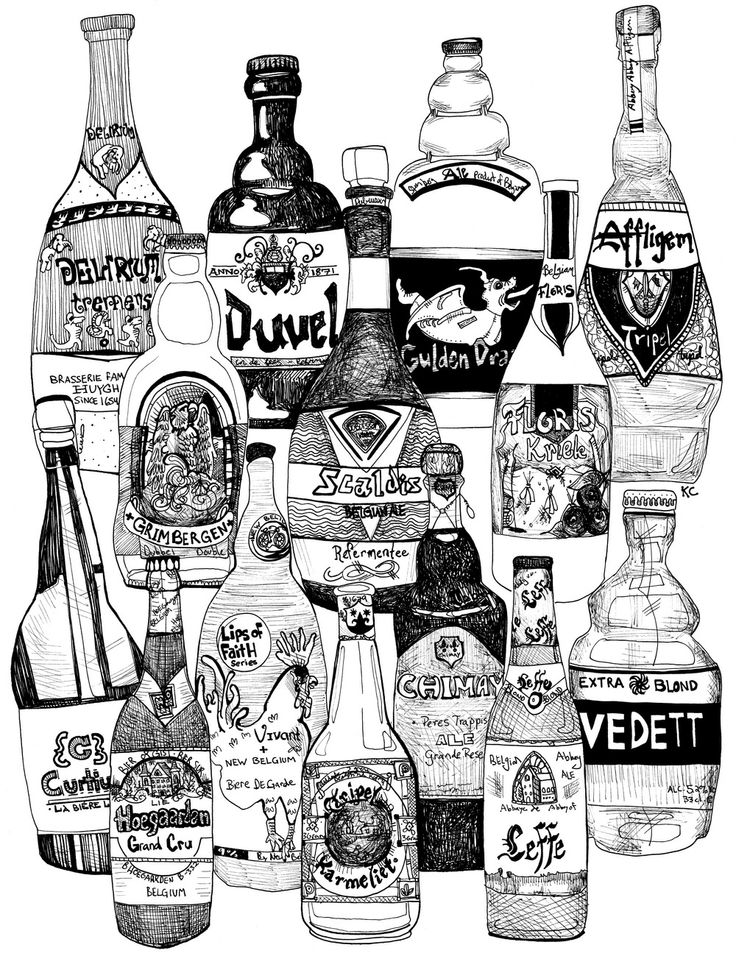
\includegraphics[height=5cm]{beerbottles}};
\end{tikzpicture}

Erilaisia oluttyylejä löytyy maailmasta lukuisia. Oluiden erilaisuuteen vaikuttavat useat eri tekijät. Mäskäyksessä käytetty mallas luo oluelle rungon ja antaa oluelle värin. Humaloinnilla voidaan vaikuttaa oluen aromeihin ja katkeruuteen. Tärkeä osa on myös hiivalla, joka vierrettä käyttäessään luo omat arominsa valmiiseen tuotteeseen.

Pelkästään esimerkiksi oluen värin tai tuoksun perusteella oluita on lähes mahdotonta luokitella. Mainitut ominaisuudet ovat vain pieniä osia tuosta monipuolisesta kokonaisuudesta, johon sisältyy myös valmistustekniikan lisäksi esteettisiä piirteitä. Esimerkiksi eri oluiden nauttimiseen tarkoitetut lasit ovat parhaimmillaan silmää hiveleviä taideteoksia.

Objektiivisin mahdollinen jako on erottaa toisistaan pinta- ja pohjahiivaoluet. Ero syntyy käymisen aikana: pintahiiva nimensä mukaisesti nousee käymisastian pinnalle, pohjahiiva vastaavasti laskeutuu sammion pohjalle. Pohjahiivaoluet vaativat matalamman käymislämpötilan, ja niiden käyminen on täydellisempää. Lopputuloksena on kirkas ja pehmeäarominen lager-olut. Pintahiivaoluet eli alet käyvät korkeammassa lämpötilassa ja ovat maultaan lagereita vivahteikkaampia. Pintahiivaoluiden monipuolisuus on täysin ylivoimainen lagereihin nähden, mutta valmistus- ja kulutusmäärissä lagerilla on maailmanlaajuisesti lähes monopoliasema. Oluttyylien rikkauden ylläpito lepääkin hyvin pitkälti pienpanimoiden ja asialleen omistautuneiden harrastajien hanoilla.

Seuraavassa luetellaan tunnetuimpia oluttyylejä näille ominaisine piirteineen.

\section{Pintahiivaoluet (alet)}

Ale on yleisnimitys pintahiivalla käytetyille oluille. Nopeahko käyminen 15--20 asteessa jättää olueeseen käymättä jääneitä sokereita, ja ale-oluita kuvataan usein hedelmäisiksi. Ale voi olla värillään yhtä hyvin kullankeltaista, punertavaa, kuin lähes läpinäkymättömän tummaa.

\subsection*{Ale (Belgia)}

Belgia on yksi merkittävimmistä olutmaista. Belgiassa toimii yli sata panimoa, jotka valmistavat yli tuhatta eri olutmerkkiä. Kaupallisten panimoiden valmistamat alet voidaan värinsä mukaan jakaa karkeasti kolmeen eri ryhmään. Blondet ovat nimensä mukaan vaaleimpia, alkoholipitoisuudeltaan n. 6--8\%, aromikkaan humaloituja ja maultaan täyteläisen maltaisia. Ambree-oluet ovat väriltään hieman punertavampia, maltaisempia, mutta vahvuudeltaan blonden luokkaa. Brune-oluet jäljittelevät maineikkaita tummia luostarioluita, eli saattavat olla vahvuudeltaan pari prosenttiyksikköä edellisiä korkeampia sekä makean maltaisia, jopa karamellimaisia. Myös vaaleat alet saattavat olla alkoholipitoisuudeltaan hyvinkin vahvoja, näistä hyvänä esimerkkinä kuuluisa oluiden ''paholainen'' 8,5-prosenttinen Duvel. Eräs mainittava oluttyyli on myös ns. flaamilainen ruskea/punainen olut (flemish brown/red ale), jolle pitkä säilytys tammitynnyrissä mikrobien toiminnan ansiosta antaa hyvinkin happaman maun. Joskus happamuuden tasoittumiseksi sekoitetaan vanhaa ja nuorta olutta keskenään, joskus olut saatetaan maustaa marjoilla, mikä on hyvin tavallista Belgiassa. Tyylin edustajia ovat mm. Rodenbach ja Liefmans Goudenband.

\subsection*{Ale (Iso-Britannia)}

Britannia on eräs merkittävimmistä ale-oluiden valmistajista. Britanniasta ovat lähtöisin niin bitter, porter, stout, kuin ''elävä'' real alekin. Lisäksi oluttyyleille on annettu lukuisia täsmentäviä lisänimiä, kuten pale ale, mild ale, Scottish ale, cream ale\ldots

\subsection*{Alt}

Saksalainen pintahiivaolut, joka kuitenkin kypsytetään pohjahiivaoluen tavoin viileässä. Nimi alt tarkoittaa vanhaa, viitaten oluenvalmistuksen perinteikkyyteen. Alt-olut on maltaista ja katkerahkoa. Väriltään alt on usein tummanruskeaa tai hieman vaaleampaa.

\subsection*{Barley wine}

Vahva pintahiivaolut (alkoholipitoisuus usein yli 10\%), jolla ei kuitenkaan nimestään huolimatta ole mitään tekemistä viinin kanssa. Valmistetaan lähinnä Brittein saarilla. Barley winet ovat maultaan erittäin monivivahteisia ja niitä suositellaan mm. jälkiruokaoluiksi ja talvi-iltojen lämmittäjiksi. Useimmiten barley winet ovat väriltään hyvin tummia, multa niitä valmistetaan myös vaaleina versioina.

\subsection*{Bitter}

Bitter-nimikkeellä on alun perin erotettu voimakkaasti humaloidut eli nimensäkin mukaisesti katkeran makuiset, kuivahkot alet miedosti humaloiduista. Bitter alet ovat väriltään kullankeltaisia tai usein punertavia.

\subsection*{Kölsch}

Kölsch on altin tavoin saksalainen pintahiivaolut ja ne ovat läheisiä sukua toisilleen. Kölsch on kuitenkin värillään hyvin vaaleaa. Aitoa kölsch-olutta saadaan valmistaa ainoastaan Kölnin seudulla, Saksassa. Kölschiä suositellaan kesäisen janon sammuttajaksi..

\subsection*{Luostarioluet}

Luostarioluilla ei ole tyylillisesti yhtenäistä tekijää. Munkkien luostareissa valmistamat oluet on kuitenkin usein niputettu saman nimikkeen alle. Lähes aina luosiarioluet ovat ale-lyyppisiä, maultaan monivivahteisia ja alkoholipitoisuudeltaan korkeita. Luostareissa valmistetut oluet jaetaan usein kolmeen luokkaan: Enkel-oluet on tarkoitettu luostarin omaan käyttöön. Enkeliä vahvempaa tummaa ja makeahkoa olutta kutsutaan dubbeliksi ja kaikkein vahvinta, vaaleaa ja usein hyvin katkeraakin olutta kutsutaan trippeliksi. Kuuluisimpia luostarioluita ovat aidot trappistioluet. Merkittäviä luostariolutmaita ovat mm. Belgia ja Saksa. Nykyään moni luostari on kuitenkin myynyt nimensä kaupallisten ja maallistuneitten panimojen käyttöön.

\subsection*{Pale ale}

Nimestään huolimatta pale ale ei ole mitenkään kalpeaa, vaan saattaa väriltään olla jopa pronssin vivahteista. Nimi on alun perin tarkoitettu erottamaan vaaleampi olut lähes mustista portereista ja stouteista. Merkittäviä pale aleja ovat mm. india pale ale (IPA), joka on aikoinaan kehitetty vientiolueksi Intiaan. Kestääkseen pitkän merimatkan siihen lisättiin runsaasti oluen säilyvyyttä parantavaa humalaa. Korkea katkerohumalapitoisuus antaa nykyäänkin IPA-oluille niiden ominaisen maun. American pale ale (APA) on IPA:n tavoin voimakkaasti humaloitua, mutta humalointiin käytetään amerikkalaisia lajikkeita, kuten Cascadea, joka antaa oluelle sitrusmaisen aromin.

\subsection*{Porter}

Porter on tarinan mukaan saanut nimensä Lontoolaisen rautatieaseman kantajien (porter) mukaan. Porter on värillään lähes musta, maltainen ale-olut, joka voi olla aromiltaan makeahko tai karvaan paahtunut. Tyyliltään hyvin lähellä stoutia.

\subsection*{Real ale}

Aito, ''elävä'' olut on eräs brittien ylpeyksistä. Real ale kypsyy samassa tynnyrissä, josta se tarjoillaan. Real alessa on vain sen oma käymisessä syntynyt hiilihappo, joten se joudutaan laskemaan tuoppiin käsin pumppaamalla. Koska avatussa tynnyrissä olut joutuu tekemisiin hapen kanssa, säilyy real ale juomakelpoisena vain muutaman päivän ajan. Koska oluen maku muuttuu tynnyrissä koko ajan, eivötkä kaksi eri tynnyriä koskaan maistu täysin samalle, on perusteltua puhua elävästä oluesta. Real ale ei sinänsä ole oma oluttyylinsä, usein tynnyreistä löytyy bitteriä tai pale alea, joskus jopa vahvaa barley wineä. Helsingistä saa säännöllisesti real alea muutamista olutravintoloista.

\subsection*{Saison}

Nimensä puolesta saison viittaa kausiolueen. Alun perin saisonia ovat valmistaneet Belgian ranskankieliset vallonit. Olut pantiin talven ja viileän kevään aikana ja varastoitiin odottamaan kesää. Säilyvyyden vuoksi saison on runsaasti humaloitua. Pitkä varastointi myös antaa olueen happamuutta ja erilaisia makuvivahteita. Saisonit ovat usein erittäin runsashiilihappoisia ja erilaisten mausteiden käyttö on yleistä. Hyvänä esimerkkinä saisoneista mainittakoon Saison Dupont.

\subsection*{Stout}

Stout luotiin aikanaan porterin tummemmaksi ja täyteläisemmäksi versioksi. Ajan myötä näiden kahden tyylin raja on hämärtynyt. Panimot nimeävät tuotteitaan omien mieltymystensä mukaisesti. Porterien tapaan stoutit ovat hyvin tummia, paahteisen maltaisia tai joskus makeahkoja, jopa suklaisia. Kuuluisin stout on kuiva, irlantilainen Guinness. Kotimainen Koff Porterkin itse asiassa edustaa tyyliltään imperial stoutia.

\subsection*{Trappist}

Trappistioluet kuuluvat arvostetuimpiin luostarioluihin, sillä ne todellakin ovat valmistettu luostareissa, trappistimunkkien valvonnan alaisuudessa. Tällä hetkellä kuusi belgialaista luostaria, Achel, Chimay, Orval. Rochefort, Westmalle ja Westvleteren saavat kantaa pullojensa etiketeissä aitouden takaavaa ''Authentic trappist''-symbolia. Myöskään trappistioluet eivät tyylillisesti ole yhteneviä: Achelilla ja Westmallelta löytyvät omat dubbel ja trippel -oluet, Chimayn, Rochefortin ja Westvleternin erikoisuuksina ovat tummat, alkoholipitoisuuksiltaan erittäin vahvat, maultaan monivivahteiset, lähes portviinimäiset oluet. Orvalin valikoima rajoittuu yhteen, runsaasti humaloituun, punertavaan ale-olueen.

\subsection*{Vehnäoluet (saksa)}

Oluen perusraaka-aineen, ohramaitaan, ohella on keksitty käyttää mm. vehnää. Vehnäoluita (weizenbier, weissbier) on valmistettu etenkin Etelä-Saksassa, Baijerissa. Vehnäoluen tunnusomaisia aromeja ovat mm. banaani ja neilikka. Suodatettua, kirkasta vehnäolutta nimitetään kristallklariksi tai kristallweizeniksi. Se on maultaan pehmeää ja puhdasta ilman hiivan antamaa makua. Suodattamaton hefeweizen on sameaa ja maultaan mausteisempaa. Täyteläiseen dunkelweizeniin on lisäksi käytetty tummaa ohramallasta. Erittäin vahvoja vehnäoluita nimitetään vehnäbockeiksi (weizenbock). Vehnäoluet ovat usein runsashiilihappoisia ja sopivat mainiosti esimerkiksi kesäisiksi terassioluiksi.

\subsection*{Witbier}

Belgiassa on syntynyt oma vehnäoluttyylinsä, jonka nimi suomentuu valko-olueksi (wit-bier, biere blanche) viitaten oluen samean vaaleaan ulkonäköön. Valmistuksessa käytetään mallastamatonta vehnää sekä usein mausteita, kuten korianteria ja appelsiininkuorta. Tunnetuin witbier lienee belgialainen Hoegaarden.

\section{Pohjahiivaoluet (lager)}

\subsection*{Bock}

Bock on nimitys vahvalle täysmallaslagerille. Nimi tulee luultavimmin Einbeckin kaupungista, jossa bock-olutta alun perin lienee pantu. Bock tarkoittaa myös pukkia, joten tämä selittää monissa olutetiketeissä esiintyvät sarvipäät. Vahvaa bock-olutta nimitetään usein doppelbockiksi (tupla-bock). Bock voi olla väriltään kullankeltaista tai hyvinkin tummaa, maultaan maltaista ja usein vahvuutensa takia alkoholimaista. Maukas talvinen lämmittäjä on esimerkiksi doppelbock Ayinger Celebrator.

\subsection*{Lager}

Lager on yleisnimitys tavalliselle pohjahiivaoluelle. Kotimaiset Karhu, Koff, Karjala, Olvi ja Lapin Kulta ovat esimerkkejä miedosti humaloiduista, helposti juotavista, ja kuluttajien suosimista lager-oluista. Täyteläisempää makua edustavat esim. Tšekki-lagerit Velkopopovicky Kozel ja Budejovicky Budvar.


\subsection*{Märzen}

Märzen-nimi tulee saksan kielen maaliskuuta tarkoittavasta sanasta März. Tämä alun perin maaliskuussa pantu, maltainen, meripihkanpunainen lager kuitenkin nautitaan vasta syksyllä Oktoberfestin yhteydessä, minkä vuoksi olutta kutsutaan myös Oktoberfestbieriksi. Aikoinaan kesä oli liian lämmintä aikaa panna olutta, joten maaliskuussa tehtiin isoja satseja kesän varalle ja nämä sitten juotiin juhlallisin menoin loppuun syksyn tullen.

\subsection*{Pilsner}

Pilsner (pils, pilsener) on saanut nimensä tšekkiläisen Plzenin kaupungin mukaan (saksaksi Pilsen), jossa vuonna 1842 kehitettiin alkuperäinen, kullankeltainen pilsner-olut, Pilsner Urquell. Pilsnerin erottaa tavallisesta lagerista voimakkaampi humalointi, tosin panimot saattavat nimetä jälleen tuotteitaan pilsnereiksi omien mieltymystensä mukaan. Vastoin suomen kieleen juurtunutta yleistä käsitystä, pilsneri ei siis tarkoita ykkösolutta.


\section{Muut}

Vaikka useimmiten oluet voidaan käymisprosessinsa perusteella niputtaa joko pinta- tai pohjahiivaoluihin, on olemassa muutama poikkeus. Merkittävimpänä belgialainen, villihiivan käyttämä lambic-olut, jonka perinteet ovat ajalta, jolloin hiivaa ei tunnettu. Myös suomalainen sahti on yksi vanhimmista primitiivisistä oluttyyleistä.

\subsection*{Lambic}

Aidon lambic-oluen valmistuksen kerrotaan olevan mahdollista vain talviaikaan Senne-joen laaksossa, Brysselin länsipuolella. Lambicin valmistukseen käytetään vähintään 30\% mallastamatonta vehnää ja humalaa vain säilöntäaineena. Keitetty vierre pumpataan yöksi jäähtymään panimon ullakolle avonaiseen jäähdytysaltaaseen, jossa ilmassa leijailevat villihiivaitiöt iskevät vierteeseen ja saavat aikaan spontaanin käymisreaktion. Tämän jälkeen olut lasketaan tammisiin tynnyreihin, joissa käyminen jatkuu ja joissa olutta varastoidaan kahdesta kolmeen vuotta. Lambicit eroavat maultaan muista oluista huomattavasti, ja niiden erityispiirre on voimakas happamuus. Harvemmin varastoitua lambicia juodaan sellaisenaan, vaan eri variaatioita saadaan sekoittamalla eri-ikäisiä lambiceja keskenään tai maustamalla olut marjoilla. Gueuze (geuze) on sekoitus vanhaa sekä nuorta, vielä hiilihappoista ja erittäin hapanta lambicia. Kriek on kirsikoilla, ja framboise (frambozen) vadelmilla maustettua lambicia. Makeahkoa faroa saadaan lisäämällä lambiciin kandisokeria, joka saa aikaan voimakkaan jälkikäymisen.

Nykyään moni panimo on hylännyt lambiciin liittyvän käsityöperinteen ja lähtenyt hyödyntämään ideaa kaupalliseen suuntaan. Monet lambicit ovat nykyään makeita ja hyvin virvoitusjuomamaisia, myöskään marjaoluihin ei käytetä aitoja marjoja, vaan makeita esansseja. Aitoa perinnettä pitävät silti yllä ainakin Cantillonin ja Drie Fonteinenin panimot.

\subsection*{Sahti}

Ei ole täysin selvää, pitäisikö sahti laskea oluttyyliksi vai täysin omaksi juomakseen. Suomalainen, ohra- ja ruismaltaasta pantu, katajalla maustettu ja leivontahiivalla käytetty sahti on kuitenkin lambicin ohella yksi vanhimmista oluttyyleistä. Sahti eroaa muista oluista siinä, että sahtivierrettä ei keitetä. Tämän takia sahti säilyy parhaimmillaankin vain muutamia viikkoja.

Sahtia on perinteisesti valmistettu juhla- ja talkooväkeä varten. Sahdinvalmistuksen perinnettä vaalii muun muassa Suomen sahtiseura\footnote{\url{http://www.sahti.org/}}.

\section*{Lähteet}

\begin{itemize}
\item{Josh Levenihal - Maailman oluet, Könemann, 2000}
\item{Kari Likovuori - Brysselin parhaat olutravintolat. Perinteisen oluen seura, 2003}
\item{Michael Jackson - Suuri Olutkirja, Gummerus, 1990}
\item{Michael Jackson - Olutta, Otava, 2002}
\item{Perinteisen oluen seura, http://www.posbeer.org}
\end{itemize}

\chapter{Oluen maistaminen ja juominen}

\begin{tikzpicture}[remember picture,overlay]
\node[anchor=east,inner sep=0pt] at (current page text area.east|-0,6cm) {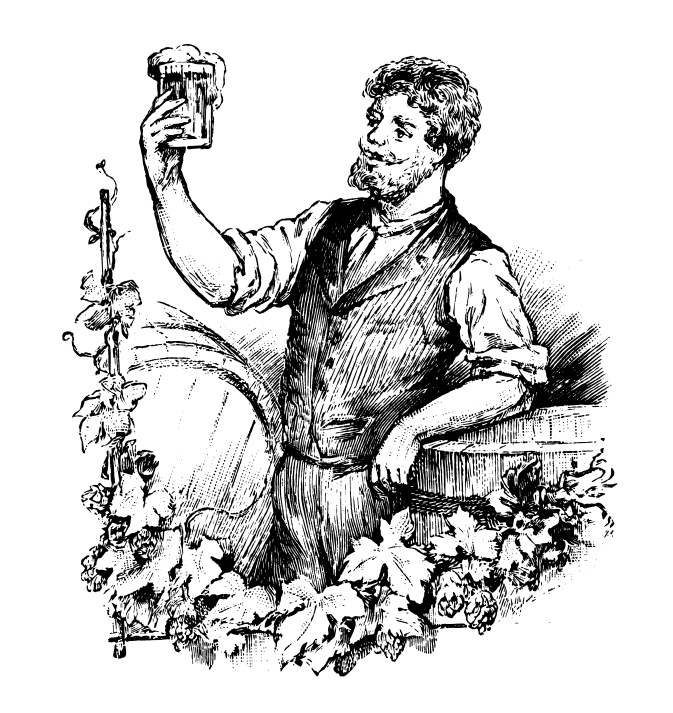
\includegraphics[height=5cm]{beertasting.jpg}};
\end{tikzpicture}

\section{Johdanto}

Oluen maistaminen ja juominen on hyvin subjektiivinen kokemus. Ei ole olemassa yhtä oikeaa lapaa nauttia oluesta, on vain hyviä neuvoja ja suosituksia, joita noudattamalla oluen nauttimisesta tulee entistäkin miellyttävämpää. Tässä luvussa esitetään joitain hyväksi havaittuja vinkkejä oluen juomiseen sekä oluesta nauttimiseen liittyviä hyviä tapoja.

Oluen maun kuvaileminen eksakteihin termeihin ja muuttujiin tottuneelle insinöörille saattaa osoittautua vaikeaksi. Toisaalta samaa tilannetta kuvaavan runoilijan teksti voi olla vieläkin vaikeampaa ymmärtää. Kun halutaan kuvailla toiselle oluen makua ja luonnetta, joudutaan turvautumaan ennalta sovittuihin termeihin. Samaan ongelmaan törmätään olutta arvostellessa, ja laitettaessa eri oluita arvojärjestykseen erilaisissa kilpailuissa. Makujen, niin toivottujen kuin virhemakujenkin, tunnistamisessa ja nimeämisessä käytetään usein apuvälineenä flavoripyörää.

Arvostelua ja kilpailuja lukuun ottamatta oluenjuonnin päätarkoitus on olla hauskaa ja rentoa. Makoisalla tuopillisella voi palkita itsensä hyvän tai huonon työpäivän jälkeen. Olut sekä rentouttaa että piristää.Olut on myös oiva seurustelujuoma.

\section{Oluen valinta}

Oikeaan tilanteeseen kannattaa valita oikea olut. Kuumana kesäpäivänä terassilla maistuu erilainen olut kuin joulun tienoilla hankien keskeltä lämpimään tupaan tullessa. Myöskään kalliita luostarioluita ei välttämättä kannata kipata pikkutunneille venähtäneiden juhlien jatkoilla. Olutharrastuksen edistyessä oppii ennen pitkää, mistä oluesta pitää ja mistä ei. Rahojaan ei tietenkään kannata tuhlata olueen, jonka mausta ei pidä. Alkuun oluen valinnassa pääsee POLKUn ''Ota oikea olut''-esitteen avulla. Yleisenä ohjenuorana voidaan pitää, että kevyeen tilanteeseen sopii kevyt olut ja raskaaseen raskas.

\section{Oluen nauttimislämpötila}

Nauttimislämpötila vaikuttaa oluen makuun huomattavasti. Tätä voi kokeilla maistamalla samaa olutta kylmänä, viileänä ja lämpimänä. Liian kylmästä oluesta on hyvin vaikea maistaa yhtään mitään. Onneksi liian kylmän oluen lämmittäminen on helppoa -- siirtää pullot ajoissa huoneenlämpöön. Usein olutravintoloissa pullot säilytetään nauttimisen kannalta liian kylmässä. Tällöin kannattaa pyytää olut pullossa pöytään ja antaa sen lämmetä. Jos olut on liian lämmintä, jotkut maut voivat peittää alleen toisia makuja eikä olut maistu tasapainoiselta.

Monien olutpullojen etiketissä on mainittu sopiva tarjoilulämpötila. Jos näin on, noudata sitä. Nyrkkisääntönä tummat ja vahvat oluet tarjoillaan lämpimämpänä kuin vaaleat ja miedot. Ääripäinä mainittakoon välimeren maissa kesäkuumalla tarjoiltava miltei jäähileinen kevyt lager seka Britannialainen erikseen yli huoneenlämpöiseksi lämmitetty stout\footnote{Goscinny \& Uderzo: Asterix Britanniassa, Sanoma Oy 1971}.

Eri lähteissä esitetään oluttyypeille erilaisia lämpötilasuosituksia. Seuraavassa taulukossa muutamia niistä:


\begin{table}[ht]
\centering
\begin{tabular}{| l | c |}
\hline
Oluttyyli & Lämpötila \\
\hline
Tummat ja vahvat alet & 16 \degree C \\
Stoutit, portterit & 14 \degree C \\
Brittiläistyyliset alet, IPAt & \\
muut pale alet, bitterit & 12 \degree C\\
Vehnäoluet, APAt, lambicit & 9 \degree C \\
Tummat ja/tai vahvat lagerit & 8 \degree C \\
Kevyet lagerit, pilsnerit & 7 \degree C tai alle \\
\hline
\end{tabular}
\caption{Taulukko 1: Oluen tarjoamislämpötiloja}
\end{table}

Kuitenkin jokainen juo oluensa sen lämpöisenä kuin siitä pitää ja yllä olevista suosituksista poiketaan usein. Esimerkiksi Guinnessin stouttia on maailmalla saatavilla myös ''Super Cold''-hanoista 1--3 asteisena.

\section{Olut juodaan lasista}

Olut kannattaa juoda lasista. Joissain tilanteissa, esimerkiksi pussikaljoitellessa, on pullosta tai tölkistä juominen on suotavaa mutta tällöinkin hieman vulgaaria. Tavallinen puolen litran suora lasituoppi tai -kolpakko sopii suurimmalle osalle oluista. Jotkut oluet suositellaan juotavaksi erikoisemmasta lasista -- esimerkiksi luostarioluet yleensä juodaan maljamaisesta lasista. Saksalaistyyppistä lageria voidaan juoda kivituopista ja tukevaa alea tinatuopista. Marjaolut voidaan hyvin juoda isosta punaviinilasista. Sahti juodaan luonnollisesti katajahaarikasta, josta irtoaa juomaan miellyttävä kataja-aromi. Joihinkin olutmerkkeihin liittyy perinteitä juoda olut erikoisesta lasista. Tunnetuin näistä lienee belgialainen Kwak, joka tarjoillaan ajurinlasista.

Olutlasin on oltava riittävän iso, että siihen mahtuu oluen lisäksi myöskin oluen vaahto. Vaahto on tärkeä, koska se suojaa olutta väljähtymiseltä. Lasin on myös oltava ilmiselvästi puhdas. Likainen lasi on ruma, ja rasva- tai pesuainejäämät voivat maistua oluen läpi tai haitata vaahdon muodostumista. Olut lasketaan lasiin kursailematta, kuitenkin niin ettei se kuohu yli. Jos olut vaahtoaa voimakkaasti, olut kannattaa kaataa lasin reunaa pitkin. Tämä hillitsee vaahtoamista. Erityisesti kotiolut on tärkeää kaataa lasiin yhdellä kallistuksella. Jos pullon joutuu nostamaan välillä pystyyn, sekoittuu hiiva pullon pohjalta olueen. Hiivaa ei haluta lasiin kuin poikkeustapauksissa -- yhtenä näistä mainittakoon suodattamaton vehnäolut.

\section{Oluen arviointi alkaa ulkonäöstä}

Oikein laskettu tuoppi on kaunis. Oluen ulkonäön ihailemiseen kannattaa uhrata aikaa, koska se kertoo oluen luonteesta miltei yhtä paljon kuin makukin. Huomiota kannattaa kiinnittää oluen väriin (vaalea, tumma, punertava, pikimusta?), vaahtoon (vahva, heikko, tiivis, hento, pysyvä, nopeasti laskeutuva?) sekä oluen kirkkauteen (kirkas, samea). Eri ominaisus saattaa olla yhdessä oluttyypissä virhe ja toisessa toivottu ominaisuus. Esimerkiksi lagerin kuuluu olla kirkasta ja suodattamattoman vehnäoluen sameaa. Vaahdon pitää olla stoutissa vahva mutta kevyessä bitterissä heikompi. Jos ulkonäössä on jotain pahasti pielessä, esimerkiksi jos suodatettu olut on sameaa, saattaa olut olla pilaantunutta.

\section{Tuoksu}

Ennen maistamista olutta kannattaa haistaa. Nenä aistii aromeja, joita ei välttämättä makuaistilla havaitse. Tuoksussa voi huomata maltaiden aiheuttaman makean ja tukevan hajun, hiivaan liittyvät hedelmäaromit tai pistävän humalan tuoksun. Tummissa porttereissa tuoksuu paahtunut mallas, tummissa legereissa makeampi mallas. Pilsnereiden tuoksusta erottaa aromihumalan, ja real aleissa tuoksuvat usein hiivan hedelmäiset käymisaromit kuten omena, appelsiini tai banaani. Lisää tuoksujen nimiä ja adjektiiveja tuoksun kuvaamiseen voi etsiä flavoripyöristä.

Jos olut ei tuoksu hyvältä, se tuskin maistuukaan hyvältä. Sen sijaan makuhermoja kutkuttava tuoksu lisää odotuksia tulevasta kulauksesta.

\section{Vihdoinkin, maku}

Kun tuoppia on riittävän kauan katseltu ja nuuhkittu, siitä otetaan reipas kulaus. Olutta otetaan suuhun tarpeeksi, niin että olut levittyy koko suun alueelle. Jotkut maistajat neuvovat puraisemaan olutta nimenomaan oluen levittämiseksi koko suuhun. Hampaat ja suun etuosa rekisteröivät makeuden, joka on peräisin maltaista. Joidenkin oluiden happamuus tai humalan kirpeys supistavat suun sisäpintoja. Olut nielaistaan ennenkuin erittyvä sylki vesittää sen. Olutta ei siis jäädä pyörittämään suussa kuten viiniä -- eikä sitä hyvänen aika ainakaan sylkäistä pois! Humalan katkeruus alkaa tuntua suun takaosassa muutaman sekunnin kuluttua nielaisemisesta. Lopuksi suuhun jää jälkimaku. Kuvailuja maulle kannattaa myöskin etsiä flavoripyörästä.

Varsinaisen maun lisäksi olutta maistaessa kannattaa kiinnittää huomiota suutuntumaan. Onko hiilidioksidia liikaa vai liian vähän? Tuntuuko olut täyteläiseltä suussa?

Kuten ulkonäössä ja tuoksussakin, jotkut maut saattavat olla toisessa oluessa toivottuja ja toisessa virheitä. Esimerkiksi mainittakoon diasetyyli, jota voidaan pitää virheenä joissain oluissa ja hienona aromina toisissa. Diasetyyli syntyy käymisen sivutuotteena, ja sen makua voidaan kuvailla voinkaltaiseksi. Ylenpalttinen katkerohumala sopii toki bittereihin, mutta vehnäoluesta toivoisi maistavan muutakin kuin katkeroa.

\begin{figure}[t]
\centerline{
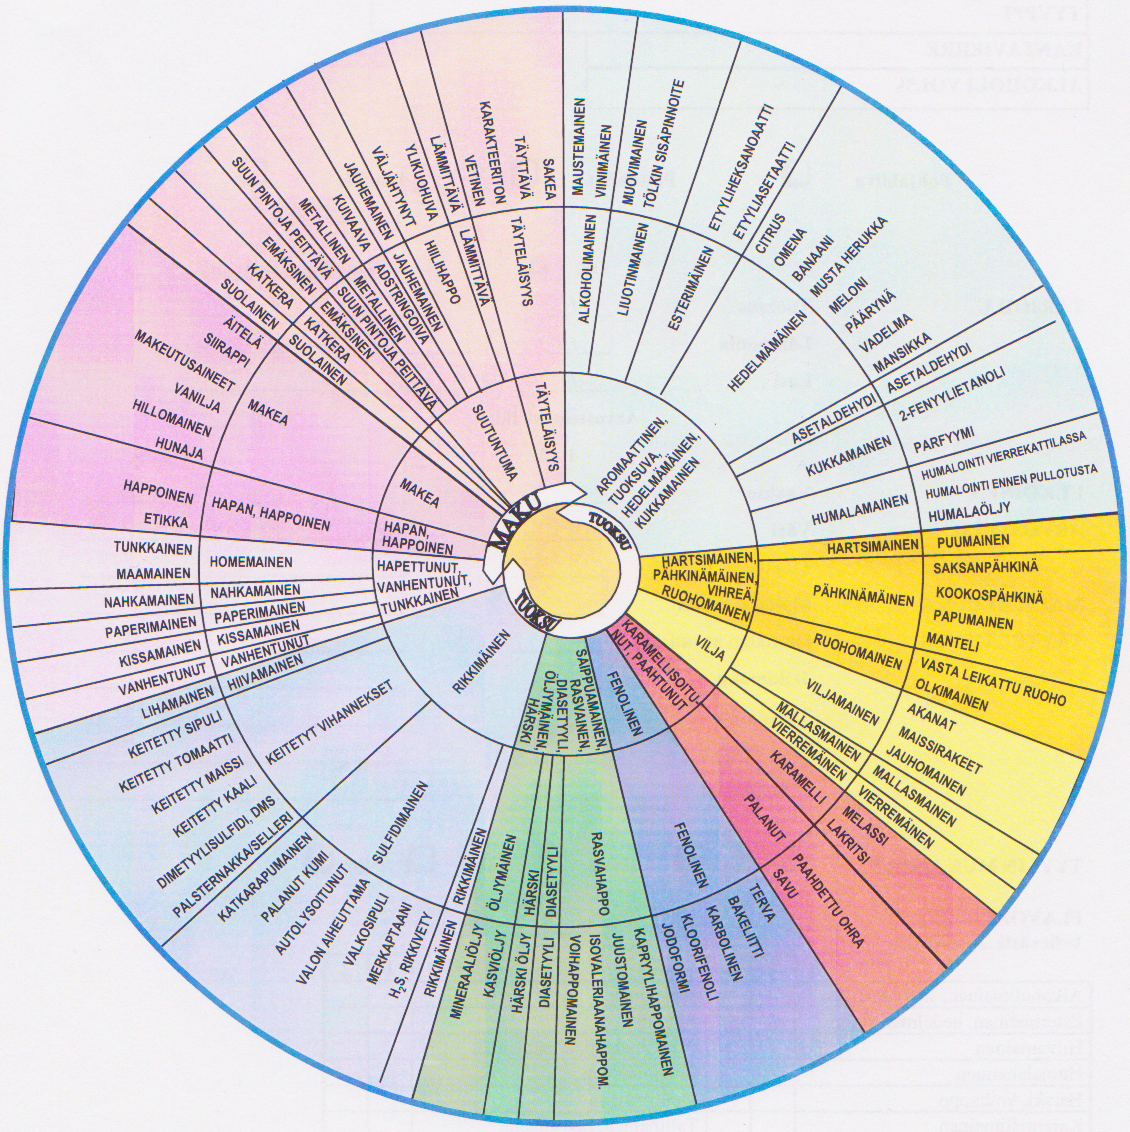
\includegraphics[width=10cm]{flavoripyoracropped.png}
}
\caption{Kuva 1: Flavoripyörä}
\end{figure}

Puhtaassa oluessa maistuu mallas, humala ja alkoholi sekä muut hiivan käymistuotteet. Oluen maistamista ei voi oppia tekstiä lukemalla, vaan siinä harjautuu erilaisia oluita maistamalla. Kuitenkin eri raaka-aineiden tunnistamiseksi kannattaa maistella erilaisia maltaita ja humaloita. Kerran humalakäpyä mutusteltuaan oluenjuoja osaa yhdistää tietyn maun humalaan. Erilaiset oluenmaistajaiset ovat erinomaisia tilaisuuksia vertailla eri ihmisten erottamia makuja.

\section{Kommentointi ja puhe}

Jos olut on hyvää, tuoppi kannattaa juoda loppuun kiireettä -- kuitenkin ennen kuin olut pääsee väljähtymään. Jos olut on selvästi pilaantunutta, kannattaa siitä ehdottomasti mainita tarjoilijalle tai kaupasta ostetun pullon tapauksessa reklamoida panimolle. Kotioluen tekijät ottavat mielellään vastaan palautetta oluestaan -- kehut tuntuvat hyville ja kritiikki auttaa tunnistamaan ja korjaamaan virheitä.

Tuopillisen jälkeen on hyvä todeta, kuinka hyvää olut oikeastaan oli. Oliko se niin hyvää että sitä voisi ottaa vielä toisen? Oliko se suorastaan niin hyvää, että sitä ottaa saman tien toisen? Oliko olut kamalaa, ihan hyvää vai jumalaista? Oluen nimi kannattaa painaa mieleen tai jopa kirjoittaa muistiin -- monet oluen ystävät kantavat mukanaan pientä vihkoa, olutpäiväkirjaa, johon he tekevät muistiinpanoja oluista.

Jos haluat maistaa useampaa olutta peräkkäin, kannattaa suu kalibroida eri oluiden välissä. Tämä tehdään yleensä syömällä tai juomalla jotain miedon makuista. Vesi, vaalea leipä, suolakeksit tai ykkösolut ovat suosittuja referenssinaposteltavia. Lisäksi oluiden maistamista ei kannata aloittaa vahvimmista oluista -- katkeran bitterin jälkeen kevyen pilsnerin aromien maistaminen voi olla hyvin vaikeaa. Liian montaa olutta ei kannata maistaa peräjälkeen, koska alkoholi turruttaa makuaistin ennemmin tai myöhemmin. Jossain vaiheessa on hyvä tunnustaa itselleen, että on siirtynyt oluen maistelusta juomiseen.

\chapter{Oluenvalmistuksen teoria}

\begin{tikzpicture}[remember picture,overlay]
\node[anchor=east,inner sep=0pt] at (current page text area.east|-0,5cm) {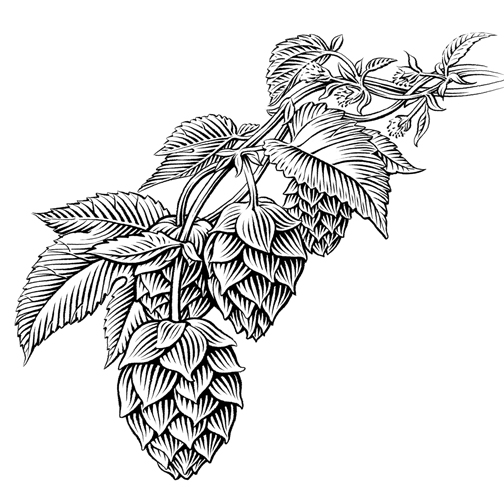
\includegraphics[height=4cm]{hops.jpeg}};
\end{tikzpicture}

\begin{figure}[th]
\centerline{

\includegraphics[width=7cm]{panokaavio.png}
}
\caption{Kuva 2: Oluenvalmistuksen periaate: Muutetaan viljan sisältämä tärkkelys sokereiksi jotka hiiva käyttää alkoholiksi. }
\end{figure}

\section{Mallastus}

Mallastuksessa viljan entsyymiaktiivisuus käynnistetään mäskäystä varten. Viljan entsyymit muuttavat tärkkelyksen sokeriksi.

\begin{figure}
\begin{tabular}{p{0.5\textwidth}p{0.5\textwidth}}
\subsection{Mallastuksen vaiheet}
\vspace{1cm}
\begin{enumerate}
\item{Liotus}
\item{Idätys}
\item{Itujen poisto}
\item{Kuivatus}
\item{Paahto}
\end{enumerate}
&
\vspace{1cm}
\begin{minipage}{.5\textwidth}
    \centering
    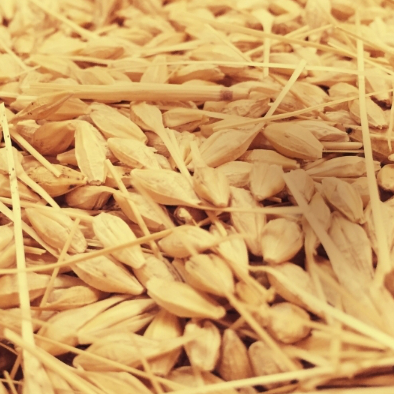
\includegraphics[width=0.8\textwidth]{unmaltedbarley}
    \caption{Mallastamatonta ohraa}
    \end{minipage} \\
\end{tabular}
\end{figure}

\begin{wrapfigure}{r}{0.35\textwidth}
  \begin{center}
    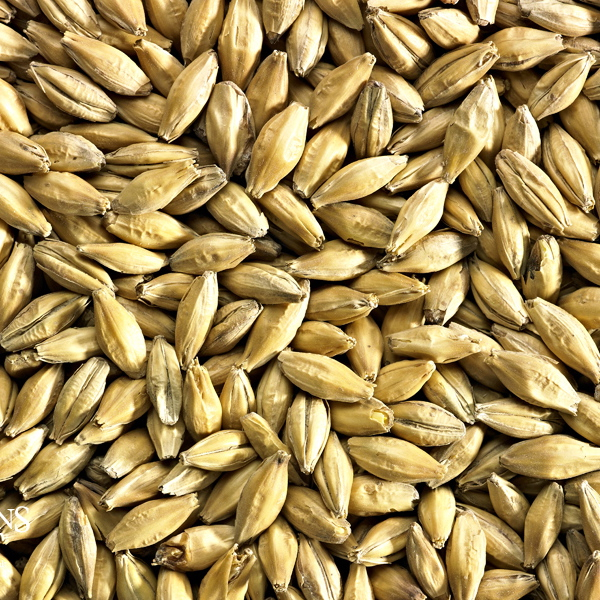
\includegraphics[width=0.32\textwidth]{pilsnermalt}
    \caption{Pilsner-mallasta}
  \end{center}
  \end{wrapfigure}
Jyvän itäessä siinä tapahtuu kaksi tärkeää reaktiota: syntyy entsyymejä ja tärkkelyksen rakenne rikkoutuu. Idätyksen yhteydessä jyvään syntyy juuri-itu, josta ei ole hyötyä oluenvalmistuksen kannalta. Tästä syystä jyvän itäminen pitää keskeyttää ennen kuin itäminen ehtii kuluttaa jyvän tärkkelyksen.

Itäminen keskeytetään kuivattamalla mallas. Samassa yhteydessä idut poistetaan. Kuivatus korkeassa lämpötilassa tuhoaa maltaan entsyymejä, sen tähden korkean entsyymipitoisuuden maltaat kuivataan matalammassa lämpötilassa kuin tummemmat erikoismaltaat. Riippuen valmisteltavasta mallaslaadusta mallas lopuksi paahdetaan.

\subsection{Yleisimmät mallaslaadut}

\begin{description}
\item[Pilsnermallas] \hfill \\
Perusmallas kaikkien oluiden valmistukseen. Kuivattu alhaisessa lämpötilassa (70--90 \degree C), joten entsyymiaktiivisuus korkea, väri vaalea, hyvä uutesaanto.
\item[Wienermallas, Münchenmallas] \hfill \\
Kuivattu korkeammassa lämpötilassa, alhaisempi entsyymiaktiivisuus, hieman tummempi väri, aromikkuampaa.
\item[Karamellimallas] \hfill \\
Kuivatusvaiheessa tärkkelyksen annetaan hydrolysoitua sokeriksi, minkä jälkeen jyvät kuivataan 150 \degree C lämpötilassa, jolloin sokeri karamellisoituu. Väreinä tumma ja vaalea, ei sisällä entsyymejä. Antaa olueeseen väriä ja makeaa makua. Ei tuota käymiskelpoisia sokereita.
\item[Värimallas] \hfill \\
Mallas paahdetaan 225 \degree C lämpötilassa, jolloin syntyy musta kahvinpapua muistuttava mallas. Antaa voimakkaan tumman värin ja karvasta makua. Ei sisällä entsyymejä eikä tuota sokereita.
\end{description}

\subsubsection*{Maltaita luokitellaan mm. seuraavilla ominaisuuksilla:}

\begin{description}
\item[Uutepitoisuus] \hfill \\
Se osa maltaan kokonaismassasta joka on muutettavissa sokereiksi. Pilsnermaltaalla > 80\%, värimaltaalla 0\%
\item[Käymisaste] \hfill \\
Kuinka suuri osa tästä maltaasta saadusta uutteesta tyypillisesti käy alkoholiksi. Pilsnermaltaalla > 80\%, värimaltaalla 0\%.

\item[Väri] \hfill \\
Pelkästään kyseisestä maltaasta valmistetun vierteen väri EBC yksiköissä (European Brewing Convention). Pilsnermaltaalla < 5, värimaltaalla > 1500.
\item[Proteiinipitoisuus] \hfill \\
Kääntäen verrannollinen uutepitoisuuden kanssa. Korkea proteiinipitoisuus heikentää uutepitoisuutta. Proteiinista ei ole hyötyä oluen kannalta, vain vähäinen määrä tarvitaan hiivan ravinnoksi.
\item[Beta-glukaani] \hfill \\
Korkea pitoisuus kasvattaa vierteen viskositeettiä ja vaikeuttaa siivilöintiä.
\item[Kosteus] \hfill \\
Korkea kosteuspitoisuus heikentää maltaan säilyvyyttä ja hankaloittaa rouhintaa.
\end{description}

\section{Mäskäys}

Maskäyksessä viljan entsyymien annetaan muuttaa tärkkelys sokereiksi, jotka liuotetaan vierteeseen. Tätä kutsutaan hydrolisoitumiseksi. Eri entsyymit ovat aktiivisia eri lämpötiloissa ja tällä voidaan ohjata prosessin kulkua säätelemällä aikaa jossa mäski on kussakin lämpötilassa.



\begin{table}[h]
\centerline{
\begin{tabular}{| l | c | l | l |}
\hline
Entsyymi & Lämpötila & Toiminta & Merkitys \\
\hline
beta-glukanaasi & 30 \degree C & Hajottaa beta- & Pienentää vierteen visko-  \\
& & glukaania & siteettia, helpottaa siivilöintiä \\
hapan proteinaasi & 45--55 \degree C & Hajottaa proteiinia & Tuottaa ravintoa hiivalle, vä-\\
& & & hentää proteiinisakkaa keito-\\ & & & ssa, kirkastaa olutta\\
karboksipeptidaasi & 60 \degree C & Hajottaa proteiinia & Tuottaa ravintoa hiivalle, vä- \\
& & & hentää proteiinisakkaa keito- \\ & & & ssa, kirkastaa olutta \\
beta-amylaasi & 62--65 \degree C & Pilkkoo tärkkelystä & Tuottaa vierteeseen käymis-\\
& & maltoosiksi & kelpoisia sokereita \\
alfa-amylaasi & 72--75 \degree C & Pilkkoo tärkkelystä & Tuottaa vierteeseen sekä käy-\\
& & & miskelpoisia että -kelvottomia \\ & & & sokereita \\
\hline
\end{tabular}
}
\caption{Taulukko 2: Mäskäyksen tärkeimmät entsyymitoiminnat}
\end{table}

Tärkkelys muodostuu pitkistä ketjumaisista ja haarakkeisista hiilihydraateista. Alfa- ja beta-amylaasientsyymit pilkkovat näitä ketjuja lyhyemmiksi sokereiksi. Hiiva pystyy käyttämään vain yhden, kahden ja kolmen sokeriyksikön mittaisia sokereita (mono-, di-ja oligosakkaridi). Tätä pidemmät sokerit ovat käymiskelvottomia ja niitä kutsutaan dekstriineiksi.

Beta-amylaasi pilkkoo ketjun päästä kahden sokeriyksikön kokoisia maltoosiyksiköitä. Beta-amylaasi ei kuitenkaan pysty jatkamaan keljun haarakohdista eteenpäin. Alfa-amylaasi pilkkoo ketjusta satunnaisesti yhden, kahden, kolmen tai useamman glukoosimolekyylin pituisia sokereita. Alfa-amylaasi katkoo tärkkelysketjua myös haarakohtien välistä, jolloin syntyy uusia ketjun päitä joita beta-amylaasi voi pilkkoa.

Pitämällä mäski pitkään beta-amylaasin toimintalämpötilassa (myös alfa-amylaasi on aktiivinen tässä lämpötilassa) saadaan mahdollisimman paljon käymiskelpoisia sokereita, jolloin saadaan korkea alkoholipitoisuus ja olut käy kuivaksi. Mikäli mäski pidetään vain alfa-amylaasin toimintalämmössä, pilkkoutuu tärkkelys satunnaisen pituisiksi ketjuiksi ja vierteeseen syntyy paljon dekstriinejä, jotka antavat oluelle runkoa ja maltaisuutta. Käymisaste on tällöin alhaisempi. Halutun oluttyylin mukaan vierre mäskätään jommassa kummassa tai sopivalla kombinaatiolla molemmissa lämpötiloissa.

On tärkeää ymmärtää että entsyymit tuhoutuvat (denaturoituvat) niiden toiminta-aluetta korkeammissa lämpötiloissa. Mikäli mäski pääsee kuumenemaan liiaksi, ei tilannetta voi enää korjata jäähdyttämällä vierrettä. Ainoat vaihtoehdot on joko muuttaa valmistettavan oluen tyyppiä tai lisätä mäskiin uutta mallasta jossa kyseistä entsyymiä edelleen on. Jos taas mäski pidetään liian pitkään beta-amylaasissa, ei olueeseen tukevuutta antavia dekstriinejä enää saada, koska kaikki tärkkelys on jo pilkkoutunut lyhyiksi sokereiksi.

\begin{table}[h]
\centerline{
\begin{tabular}{| l | l | l | l |}
\hline
Tyyli & Beta [min] & Alfa [min] & Kommentti \\
\hline
Lager & 120 & 0 & Kuivat, ohut, ei tukevuutta. Korkea\\
& & &  käymisaste  \\
Pils & 90 & 30 & Kuivahko, hieman runkoa\\
Alt & 60 & 60 & Selvästi tukevuutta, hieman makeutta \\
Tumma lager & 15 & 90 & Selkeästi makea, alhainen käymisaste \\
Stout & 0 & 120 & Erittäin tukeva runko, makeus peittyy \\
& & & värimaltaan karvauden alle \\
\hline
\end{tabular}
}
\caption{Taulukko 3: Esimerkki mäskäysohjelmista eri oluttyyleillä}
\end{table}

\section{Mäskäysmenetelmät}

\subsection{Vaiheinfuusio}

Mäskin lämpötilaa ohjataan portaittain halutun mäskäysohjelman mukaisesti. Koko mäskiannos pyritään pitämään mahdollisimman tarkasti samassa lämpötilassa. Mäskäytymistä voidaan tällä menetelmällä ohjata tarkasti. Yleisimmin käytetty menetelmä. Lämmitys voidaan suorittaa ulkoisella lämmityksellä, höyryllä, kuumalla vedellä tai muilla menetelmillä.

\subsection{Vakiolämpötila}

Koko mäskiannos pidetään koko maskäyksen ajan vakiolämpötilassa. Kaikki entsyymit eivät ole mukana tätä menetelmää käytettäessä, joten maltaan tulee olla erityisen hyvälaatuista (hyvin modifioitunutta). Käytetään yleisesti brittiläisten ale-oluiden valmistuksessa.

\subsection{Keittomäskäys}

Mäskin lämmitys tapahtuu ottamalla osa mäskistä ja kuumentamalla se kiehuvaksi ja sen jälkeen palauttamalla muun mäskin joukkoon. Yleisimmin käytetään 2- tai 3-keittomäskäystä. Keittäminen denaturoi kaikki mäskin entsyymit, jolloin mäskäysaika oleellisesti pitenee. Mäskin keittäminen antaa myös oman luonteenomaisen makunsa oluelle. Käytetään erityisesti tšekkityylisten pils-oluiden valmistuksessa.

\section{Keitto ja jäähdytys}

Mäskäyksessä saadun vierteen keitolla on monta merkitystä, tärkeimpänä niistä oluen humalointi. eli maustaminen. Keiton tarkoituksia:
\begin{itemize}
\item Entsyymien denaturointi
\item Proteiinien goakulointi
\item Veden haihduttaminen
\item Haitallisten yhdisteiden poistaminen
\item Humalointi
\item Maillard-reaktio
\item Vierteen sterilointi
\end{itemize}

Vierrettä keitetään 1--2 tuntia. Keiton yhteydessä vierteeseen lisätään humalaköynnöksen kukinnoista saatavia käpyjä. Keiton aikana humalassa olevat alfahapot liukenevat vierteeseen ja antavat oluelle katkeroa ja aromeja. Humalan alfahappopiloisuus vaihtelee 2--20\%, ja sillä on melko suuri merkitys humalan käytön kannalla.

\begin{wrapfigure}{r}{0.35\textwidth}
  \begin{center}
    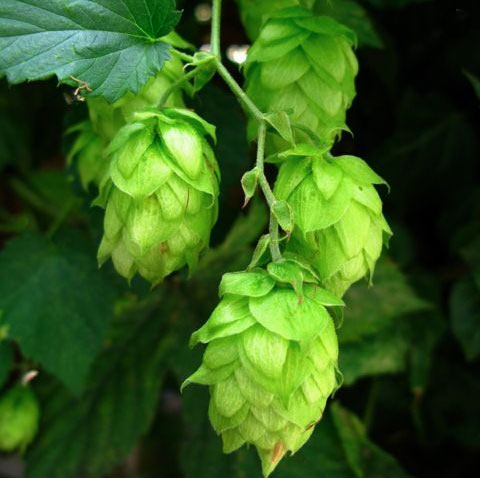
\includegraphics[width=0.32\textwidth]{hops}
    \caption{Humalakäpyjä}
  \end{center}
  \end{wrapfigure}

Humalasta liukenevat aromaattiset öljyt haihtuvat keiton aikana, joten keiton alkuvaiheessa lisättävät humalat antavat oluelle vain pistävää katkeraa makua (bitter), tätä kutsutaan katkerohumaloinniksi. 60--90 minuutin keiton aikana kaikki humalan katkeroaineet ehtivät liueta vierteeseen.

Aivan keiton loppuvaiheessa lisätyistä humalista jää vierteeseen myös aromaattisia öljyjä. Nämä antavat mausteisia, kukkamaisia ja yrttimäisiä makuja ja tuoksuja olueeseen. Tätä kutsutaan aromihumaloinniksi. Aromihumalointiin käytetään tyypillisesti alhaisen alfahappopitoisuuden (< 6\%) omaavia lajikkeita.


\begin{table}[h]
\centerline{
\begin{tabular}{| l | l | l | l |}
\hline
Lajike & Alfa [\%] & Profiili & Käyttö \\
\hline
Hallertau, saksa  & 2--5 & Mausteinen, mieto & Saksalaisissa lagereissa/pilsseissä\\
& & yrtti & \\
Saaz, Tšekki & 3--4.5 & Hienostunut, kukkai- & Tšekkilager: Pilsner Urquell\\
& & nen & \\
East Kent Goldings, & 4--6 & Pyöreä, kirpeä & Brittiläiset alet/bitterit: ESB,\\
Iso-Britannia & & &Special London ale \\
Cascade, USA & 4,5--7 & Mausteinen, kukkai- & American Pale Ale: Sierra Nevada\\
& & nen, sitrusmainen &Pale Ale \\
Chinook,  & 12--14 & Mänty, mausteinen, & Katkerohumala monenlaisiin olui-\\
USA & & hento greippi & siin, ajoittain myös aromina\\
\hline
\end{tabular}
}
\caption{Taulukko 4: Esimerkkejä joistakin humalalajikkeista}
\end{table}

Kuuma vierre pitää jäähdyttää mahdollisimman nopeasti hiivan käymislämpötilaan. Kuumassa vierteessä syntyy dimetyylisulfidia (DMS) joka antaa vierteelle keitettyjen vihannesten aromin. Keiton aikana DMS haihtuu vierteestä samaan tahtiin kuin sitä syntyy, mutta keiton jälkeen syntyvä DMS jää vierteeseen. Kuuma vierre on myös altis hapettumaan, jolloin syntyy oluen maun kannalta haitallisia oksideja. Kylmään vierteeseen liukeneva happi edistää hiivan kasvua, mutta ei tuota haitallisia yhdisteitä.

\section{Käyminen}

Hiiva muuttaa vierteen sisältämän sokerin alkoholiksi ja tekee vierteestä oluen. Hiivat jaetaan perinteisesti kahteen ryhmään:
\begin{description}
\item[Pintahiiva] \hfill \\
Käy nopeasti lämpimässä 16-24 \degree C, luottaa olueeseen runsaasti aromeja. Käytetään pääsääntöisesti kaikissa muissa oluttyyleissä paitsi lager ja pils.
\item[Pohjahiiva] \hfill \\
Käy hitaasti viileässä 5-12 \degree C, tuottaa puhtaan maun jossa ei juuri aromeja. Lager- ja pils-oluiden valmistus.
\end{description}

Hapekkaissa olosuhteissa hiiva hajottaa sokeria täydellisesti vedeksi ja hiilidioksidiksi (aerobinen aineenvaihdunta) ja saa tästä runsaasti energiaa kasvamiseen (2,87MJ/mol). Vierteen ilmastaminen ennen käymistä on tärkeää vahvan ja terveen hiivapopulaation valmistamiseksi. Kun hiiva on kuluttanut vierteestä kaiken hapen se joutuu siirtymään anaerobiseen aineenvaihduntaan, jolloin sokeri muutetaan välivaiheiden kautta etanoliksi ja hiilidioksidiksi, tästä hiiva saa energiaa vain 0,23MJ/mol. Anaerobisen käymisen varmistamiseksi tulee varmistaa ettei vierre pääse käymisen aikana hapettumaan.

Hiiva ei koskaan köytä kaikkia vierteen sokereita alkoholiksi, käymisaste vaihtelee 50--80\% välillä. Toinen hiivan ominaisuus on flokkuloituvuus, eli kuinka hyvin hiiva käymisen jälkeen pakkautuu sedimentiksi. Kotioluessa korkea flokkuloituvuus on toivottava ominaisuus, koska olutta ei suodateta ennen astiointia.

Käytännössä alkoholikäyminen ei ole koskaan puhdasta, vaan hiivan aineenvaihdunnan tuloksena oluehen syntyy paljon muitakin yhdisteitä, joilla on tärkeä osuus etenkin ale-oluiden maussa. Suurina pitoisuuksina ne kuitenkin tulkitaan käymisvirheiksi. Viileässä käyvät pohjahiivat tuottavat vain vähän sivumakuja. Merkittävimmät sivutuotteet ovat:
\begin{description}
\item[Sikuna-alkoholit] \hfill \\
Etanolia pitkäketjuisempia alkoholeja (OH-ryhmä), joilla on voimakas maku ja tuoksu (pontikka). Runsas sikunaisuus aiheuttaa päänsärkyä ja muita oireita. Pidetään käymisvirheenä.
\item[Esterit] \hfill \\
Alkoholien ja happojen muodostamia yhdisteitä, nämä saattavat antaa oluelle liuotinmaisia, hedelmäisiä tai hunajaisia aromeja.
\item[Ketonit ja aldehydit] \hfill \\
Karbonyyliyhdisteitä joista merkittävin on diasetyyli, joka antaa voimaisen, härskiintyneen maun. Asetaldehydi puolestaan antaa oluelle ruohomaisen aromin. Varastokäymisen aikana nämä kuitenkin hajoavat, joten riittävän pitkään varastoidulla kotiovella ne eivät yleensä ole ongelma.
\item[Rikkiyhdisteet] \hfill \\
Haitallisia ja epätoivottuja. Yleisin on dimetyylisulfidi (DMS), joka antaa keitettyjen vihannesten maun.
\end{description}

Pääkäyminen (primäärikäyminen) pintahiivaoluilla kestää noin viikon, jona aikana pääosa alkoholista muodostuu. Pohjahiivoilla pääkäyminen saattaa kestää kuukauden. Pääkäymisen jälkeen oluen maku ei ole vielä kovinkaan lähellä tavoiteltua lopputulosta. Varastointitankissa/astiassa olut jälkikäy (sekundaarikäyminen) ja sen makuyhdisteet kehittyvät. Kotioluen maku paranee useiden kuukausien ajan pudotuksesta.

\begin{table}[hb]
\centerline{
\begin{tabular}{| l | l | l | l | l |}
\hline
Hiiva & Lämpötila & Flokkuloituvuus & Maku & Käyttö \\
\hline 
American Ale & 15--22 \degree C & matala & Melko puhdas, rapea. & American Pale Ale \\
& & & Vähäinen hedelmäisyys. & \\
Irish Ale & 16--22 \degree C & keskimääräinen & Jonkin verran hedel- & Stout, Porter: Guin- \\
& & & mäisyyttä ja estereitä & ness, Beamish Stout \\
London ESB  & 18-22 \degree C & korkea & Maltainen, makeahko. & Britti ale/bitter Ful-\\
& & & Melko hedelmäinen, & ler's London Pride, \\
& & & diasetyyliä. & Young's \\
Bohemian Lager & 9--14 \degree C & keskimääräinen & Maltainen, hieman & Pilsner: Ayinger, \\
& & & estereitä & Sam Adam's \\
Weihenstephaner & 18--24 \degree C & alhainen & Banaaniestereitä, fenole- & Vehnäolut: Ayinger, \\
Weizen & & & ja, purkkamainen maku & Erdinger, Weihen- \\
& & & & stephaner \\
\hline
\end{tabular}
}
\caption{Taulukko 5: Esimerkkejä Wyeast-laboratorion liiivakannoista}
\end{table}
\subsection*{Lähteet}
\begin{itemize}
\item Järmälä Ari. Kotipanimomestarin käsikirja. Omakustanne 1995. ISBN 952-90-5499-8
\item Sysilä Ilkka, Ohrapellosta etiketin taakse. Omakustanne 1994. ISBN 952-90-6007-6
\end{itemize}

\chapter{Kotioluen valmistus}

\begin{tikzpicture}[remember picture,overlay]
\node[anchor=east,inner sep=0pt] at (current page text area.east|-0,5cm) {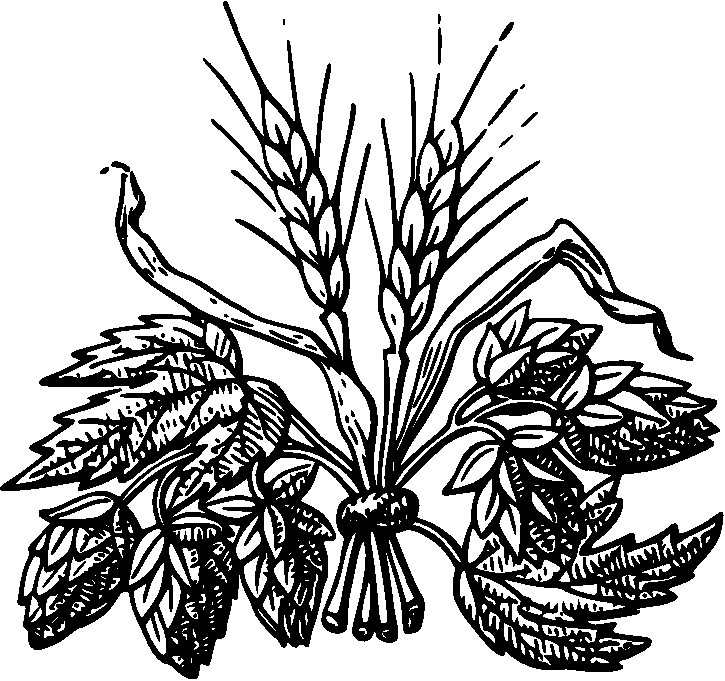
\includegraphics[height=4cm]{hopAndBarley.eps}};
\end{tikzpicture}

\section{Yleistä kotioluesta}

Kotioluella tarkoitetaan olutta, joka on valmistettu ei-kaupallisessa mielessä omaksi iloksi ja harrastuksenomaisesti. Kotiolut sinänsä voi olla yhtä hyvää ja parempaakin kuin kaupallinen olut, menetelmät ja raaka-aineet ovat samoja. Kaikkia olutlaatuja on mahdollista valmistaa kotipanimossa kunhan vain välineet, tilat ja taito ovat kunnossa. Edes valmistusmäärä ei rajaa kotiolutta. Kotona tai kerhotiloissa voidaan suhteellisen helposti valmistaa olutmääriä jotka täyttäisivät jo mikropanimon (Suomessa 150 -- 500 l keittoa kohti) määritelmän mutta olut on silti kotiolutta. Yleisimmin kotioloissa valmistettu erä on kooltaan kuitenkin 20-30 I ja lähes kaikki valmiina löytyvät reseptit on suunniteltu tähän kokoon. Reseptejä on kuitenkin helppo muokata sopimaan suuremmille tai pienemmille erille.

Tässä monisteessa keskitytään lyhyesti kotioluenpanon keskeisiin menetelmiin, välineisiin ja yleistä huomiota vaativiin asioihin. Esimerkiksi kaavoja ja laskelmia ei esitetä ollenkaan koska ne on helposti löydettävissä aihetta käsittelevistä julkaisuista. Luvussa 5 käsitellään hieman tarkemmin valmistuksen teoriaa, mutta kiinnostuksen herättyä on jokaisen aloittelevan kotipanijan syytä tutustua tarkemmin alaa käsitteleviin julkaisuihin, joita löytyy runsaasti.

\section{Hygienia}

Hyvästä hygieniasta huolehtiminen kuuluu itsestään selvyytenä jokaiseen olutpanoon menetelmästä riippumatta. Hygienialla tarkoitetaan niin laitteistojen, panotilojen kuin panijoidenkin puhtautta. Hyvinkin suunnitellun ja toteutetun panon pystyy helposti pilaamaan laiminlyömällä puhtauden tai huolimattomuudella yhdessäkin prosessin vaiheessa.

Panotilan puhtausasteeksi riittää usein perussiisteys, jossa ei lentele kärpäsiä tms. Laitteiden kanssa tekemisiin joutuvat pinnat on hyvä pyyhkiä puhdistusaineella ennen panemista. Panohenkilöstö huolehtii luonnollisesti hyvästä käsihygieniasta ja välttää räkimästä välineisiin yms.

Laitteiston peruspuhtaus on ensiarvoisen tärkeää. Pinttynyt lika vaikeuttaa tai tekee puhdistamisen mahdottomaksi ja estää näin prosessin loppuvaiheessa tarvittavan steriiliyden. Peruspuhtaus riittää laitteille, joita käytetään prosessissa keittoon asti. Keiton jälkeen kaikkien laitteiden on oltava hyvin desinfioituja! Desinfiointi voidaan suorittaa esimerkiksi kiehuvalla vedellä tai panotarvikekaupoista löytyvällä jodoforilla. Huolellinen desinfiointi tulee suorittaa vähintään käymisastialle, kannelle, vesilukolle, jäähdyttimelle, sekoituskauhalle ja lämpömittarille eli kaikelle mikä on tekemisissä jäähdytetyn vierteen kanssa.

Nyrkkisääntönä olkoon:

\begin{center}
\textbf{Puhdista aina mieluummin liikaa kuin liian vähän!}
\end{center}

\section{Valmistusmenetelmät}

Kotioluen yleisiä valmistusmenetelmiä on neljä: valmistus olutpakkauksesta, uutepano, osittaismäskäys ja mallaspano. Lisäksi näistä kaikista voi toteuttaa erilaisia variaatioita eikä mitään menetelmää tarvitse orjallisesti noudattaa. Myös kirjallisuus tulkitsee monesti menetelmiä hiukan eri tavalla, mutta pääpiirteittäin jaottelu on kuvatunlainen.

\subsection{Valmistus olutpakkauksesta}

Kotioluenvalmistus olutpakkauksesta on yleisin ja yksinkertaisin menetelmä valmistaa kotiolutta. Oluttarvikeliikkeestä saatavissa pakkauksissa on mukana kaikki tarvittavat raaka-aineet ja valmistamiseen tarvitaan vain vähän välineistöä. Pakkaus sisältää mallasuutteen joka on valmiiksi humaloitu ja erillisen kuivahiivapussin. Koska pakkausten mallasuutemäärä, yleensä 1.7 kg, on varsin pieni joudutaan tavanomaisen 23 litran erän valmistamiseksi turvautumaan lisäsokeriin. Suositeltavampi tapa olisi käyttää toista uutepurkkia, mutta tällöin kustannukset kasvavat melkoisesti.

Valmistusprosessi on mahdollisimman yksinkertainen. Mallasuutepurkin sisältö kaadetaan kattilaan, laimennetaan vedellä ja kuumennetaan noin 75 \degree C joka riittää tappamaan useimmat mikrobeista. Mallasuutetta ei ole hyvä keittää, koska siinä mukana olevat humalasta peräisin olevat aromi aineet haihtuvat helposti pois. Sama toimenpide tehdään halutulle määrälle sokeria. Raaka-aineet kaadetaan käymisastiaan johon lisätään kylmää vettä siten, että haluttu vierremäärä saavutetaan. Kun vierteen lämpötila on alle 30 \degree C voidaan joukkoon lisätä pakkauksen mukana tullut hiiva. Lopuksi koko vierre sekoitetaan hyvin ja varustetaan kannella ja vesilukolla. Käyminen tapahtuu huoneenlämmössä (20--23 \degree C).

Useimmissa olutpakkauksissa on tarkemmat ohjeet raaka-ainemääristä ja valmistusprosessista.

Menetelmän hyviä ja huonoja puolia:
\begin{description}
\item[+] Menetelmä on yksinkertainen ja vaatii vähän laitteita 
\item[+] Menetelmä on nopea
\item[--] Vierrettä ei keitetä, kontaminaatioriski suuri.
\item[--] Panijan vaikutusmahdollisuudet vähäiset
\item[--] Kidesokerin käyttö johtaa ''laihaan'' ja ''simamaiseen''
\item[--] Lopputulos ei useinkaan kovin ihmeellinen
\item[--] Uutepakkaukset ovat usein aika kalliita muihin menetelmiin verrattuna 
\end{description}
Uutepakkauksesta tehtyä olutta on helppo parantaa!
\begin{itemize}
\item Vierteen keitto
\item Sokeri pois, käytetään pelkkää mallasuutetta
\item Humaloidaan itse
\item Parempilaatuinen hiiva ja kunnollinen ''startteri''
\end{itemize}
Tarvittavat välineet:
\begin{itemize}
\item Pienehkö kattila, mieluiten kuitenkin 5--10 l
\item Kannellinen käymisastia (30 litraa jos vierrettä 25 litraan)
\item	Vesilukko
\item	Kauha
\item	Lappoletku
\item	Lämpömittari
\item	Mitta-astia
\item	Ominaispainomittari
\item	Kruunukorkkiprässi
\end{itemize}

\subsection{Uutepano eli valmistus mallasuutteesta}

Pantaessa olut mallasuutteesta saadaan huomattavasti enemmän mahdollisuuksia ja saavutetaan pakkauksia parempi lopputulos. Uutepano vastaa jo hyvin pitkälle oikeaa oluenpanoprosessia vaikkakin mäskäysvaihe jää pois. Uutepanossa käytettävä mallasuute poikkeaa pakkausuutteesta siten, että sitä ei ole humaloitu valmiiksi. Näin ollen panija joutuu (saa!) humaloida oluensa itse ja pääsee näin ollen enemmän vaikuttamaan lopputulokseen.

Mallasuutepanossa keittokattilaan lisätään ensin vettä 4/5 halutusta vierremäärästä ja tämän jälkeen mallasuutepurkkien sisältö. Vierre lämmitetään kiehuvaksi lisäten samalla vettä, jotta haluttu vierremäärä saavutetaan. Kun vierre saadaan kiehuvaksi, lisätään ensimmäiset humalat, eli ns. katkerohumalat jotka saavat olla vierteessä koko keiton ajan. Vierrettä keitetään tunnista kahteen tuntia ja keiton lopulla (15--5 min ennen loppua) siihen lisätään humalia (aromihumalat) antamaan oluelle aromikkuutta. Keiton jälkeen vierre jäähdytettään jäähdyttimen avulla mahdollisimman nopeasti hiivauslämpötilaan (noin 25 \degree C) ja lasketaan käymisastiaan. Hiivauksessa käytetään mieluiten laadukasta nestehiivaa jota varten on hyvä tehdä hiivastartteri. Nestehiivaa käytettäessä käymislämpötilalla on enemmän merkitystä ja valmistajan suosittelema lämpötila selviää hiivapakkauksesta.

Menetelmän hyviä ja huonoja puolia:
\begin{description}
\item[+] Melko yksinkertainen (ei mäskäystä)
\item[+] Panijalla monia vaikutusmahdollisuuksia (uutteet, humalointi, hiiva jne.) 
\item[+] Vierre keitetään, kontaminaatioriski pienenee merkittävästi 
\item[+] Lopputulos melko hyvä, lähellä ''oikeaa'' olutta.
\item[+] Nopeampi verrattuna mäskäämällä tehtyyn olueen.
\item[--] Vaatii ison keittokattilan ja muuta laitteistoa (jäähdytin yms.)
\item[--] Vaatii enemmän aikaa
\item[--] Vaatii enemmän taitoa
\end{description}
Tarvittavat välineet pakkauksesta valmistamisen lisäksi:
\begin{itemize}
\item Keittokattila, vähintään 30 l
\item Kaasupoltin tai muu tehokas kuumennin
\item Jäähdytin
\end{itemize}

\subsection{Osittaismäskäys}

Osittaismäskäys on menetelmänä hyvin samankaltainen kuin uutepano. Ero näillä kahdella mäskäystavalla on, että osittaismäskäyksessä mäskätään haluttu määrä mallasta mallasuutteen lisäksi jolloin saadaan lisäominaisuuksia olueen. Osittaismäskäys tehdään keittokattilassa ja yleensä käytetään vakiolämpötilamäskäystä. Keittokattilaan lisätään mäskättävästä mallasmäärästä riippuva määrä vettä joka lämmitetään mäskäyslämpotilaan. Mäskättävät maltaat laitetaan lämpöä kestävään pussiin, joka laitetaan kattilaan. Pussia pidetään mäskäyslämpöisessä vedessä haluttu aika, jonka jälkeen pussi poistetaan ja vierre kuumennetaan kiehuvaksi. Tässä vaiheessa vierteeseen lisätään mallasuute, jonka jälkeen edetään kuten uutepanossa.

Menetelmän hyviä ja huonoja puolia uutepanoon nähden:

\begin{description}
\item[+] Panijalla enemmän mahdollisuutta vaikuttaa lopputulokseen
\item[--] Vie enemmän aikaa
\item[--] Vaatii enemmän taitoa, koska tarvitaan tietämystä mäskäyksestä 
\end{description}
Tarvittavat välineet uutepanovälineiden lisäksi:
\begin{itemize}
\item Mäskäyspussi
\end{itemize}
\subsection{Mallaspano eli valmistus maltaista mäskäämällä}

Mallaspano on oluenteon perinteisin, monimutkaisin, työläin, haastavin ja ennen kaikkea antoisin menetelmä. Menetelmää käytetään, kun halutaan juuri tietynlaista olutta ja pyritään vaikuttamaan kaikkiin oluen osatekijöihin. Menetelmän opittuaan panija voi hyvällä todennäköisyydellä määrätä täysin ennalta, millaista olutta haluaa sekä tehdä kopioita tai muunnelmia kaupallisista oluista. Mikään ei estä kehittämästä vaikka omaa oluttyyliä!

Mallaspanon vaiheita käsitellään yksityiskohtaisemmin luvussa 5, joten tässä käydään prosessi läpi pintapuolisemmin.

Mallaspanoprosessi sisältää seuraavat vaiheet:
\begin{enumerate}
\item Maltaan rouhinta \hfill \\
Maltaat hankitaan esimerkiksi mallastamolta (tai oluttarvikeliikkeestä) yleensä rouhimattomina, koska niiden säilyvyys on huomattavasti parempi. Maltaat täytyy rouhia, koska käymiskelpoinen tärkkelys on jyvän sisällä. Rouhinnassa jyvä puristetaan ns. valssimyllyllä. jolloin jyvän kuori halkeaa ja vesi pääsee kosketuksiin tärkkelyksen kanssa. Kuorta eli akanaa ei kuitenkaan saa rikkoa koska sillä on tärkeä osa vierteen suodatuksessa. Maltaita voi myös ostaa valmiiksi rouhittuna, mutta saatavuus ja säilyvyys ovat heikompia.
\item Vedenlämmitys ja sisäänmäskäys \hfill \\
Varsinainen valmistusprosessi alkaa sisäänmäskäyksellä. Sisäänmäskäyksellä tarkoitetaan sitä hetkeä (veden lämpötilaa) johon maltaat tai osa niistä laitetaan. Sisäänmäskäys tapahtuu usein noin 30 \degree C lämmössä (kis. luku 5), mutta myös monia muita lämpötiloja käytetään.
\item Mäskäysprosessi \hfill \\
Sisäänmäskäyksen jälkeen siirrytään mäskäysprosessiin jossa mäskiä pidetään tietyn profiilin mukaisesti eri lämpötiloissa, (kts. luku 5)
\item	Ulosmäskäys \hfill \\
Mäskäysprosessin päättää ulosmäskäys jossa mäskin lämpötila nostetaan 78 \degree C asteeseen, jolloin entsyymitoiminta lakkaa. Mäskäys kestää tyypillisesti kaikkine vaiheineen noin 2.5 tuntia.
\item	Siivilöinti \hfill \\
Ulosmäskäyksen jälkeen mäski siivilöidään vierteeksi. Siivilöinti tapahtuu käyttäen hyväksi jyvien kuoriosia jotka muodostavat mäskäysastian pohjalle tiiviin patjan. Siivilöinnissä astian pohjalle jäävää patjaa (rapa) huuhdotaan vielä vedellä, jotta kaikki sokerit saataisiin talteen.
\item Keitto \hfill \\
Siivilöinnin jälkeen vierre lämmitetään kiehuvaksi ja aloitetaan keitto. Keitolla on monta tehtävää, joista tärkeimpänä oluen humalointi eli maustaminen (kts. 5). Keiton alussa lisätään katkeroaineita luovuttavat katkerohumalat ja keiton lopussa aromiaineita luovuttavat aromihumalat. Keitto kestää 1-2 h riippuen humaloinnista ja halutusta haihtumismäärästä.
\item Jäähdytys \hfill \\
Keiton jälkeen vierre täytyy hapettumisen ja kontaminaatioiden välttämiseksi jäähdyttää mahdollisimman nopeasti. Jäähdytys tehdään jäähdyttimellä. jonka läpi vierre lasketaan käymisastiaan.
\item Hiivaus \hfill \\
Hiivauslämpötilaan jäähdytetty vierre hiivataan hiivapanoksella, eli startterivierteellä. Startterivierre sisältää runsaasti hiivasoluja jolloin käyminen alkaa nopeasti ja tehokkaasti. Tämä on tärkeää, jotta vierteeseen mahdollisesti jääneet mikrobit eivät pääse lisääntymään.
\item Käyminen \hfill \\
Lopuksi vierre laitetaan käymään sopivan lämpöiseen paikkaan (kts. 5)
\end{enumerate}
Menetelmän hyviä ja huonoja puolia uutepanoon nähden:
\begin{description}
\item[+] Panijalla täysi vaikutusmahdollisuus lopputulokseen
\item[+] Kaikki tehdään itse
\item[+] Auttaa ymmärtämään oluen ''sielun'' ja näin kehittämään harrastusta 
\item[+] Edullinen
\item[--] Vaativa ja työläs
\end{description}
Tarvittavat välineet uutepanovälineiden lisäksi:
\begin{itemize}
\item Mallasmylly, jos maltaat rouhitaan itse
\end{itemize}
\subsection{Kaikille valmistusvaiheille yhteiset vaiheet}
\begin{enumerate}
\item Käyminen \hfill \\
Hiivauksen jälkeen olut käy hiivatyypistä riippuen viikosta kuukauteen. Tätä vaihetta kutsutaan pääkäymiseksi (kts. 5) Käymisen päättyminen havaitaan siitä, että vesilukosta tulevien kuplien väli kasvaa selvästi yli minuuttiin. Käymisen loppuminen varmistetaan ominaispainomittarilla, jonka näyttämä ei saa muuttua vuorokauden kuluessa. Ominaismittarin näyttämä on yleensä käymisen loputtua alle lukeman 1.018.
\item Astiointi \hfill \\
Pääkäymisen jälkeen olut astioidaan pulloihin, pieniin peltitynnyreihin (yleensä 5 l) tai isoihin paineastioihin (19-30 I). Astioinnin yhteydessä pulloihin ja peltitynnyreihin lisätään sokeria tai mallasuutetta jälkikäymistä varten 5-10 g litraa kohden. Astioinnissa tulee kiinnittää erityistä huomiota astioiden puhtauteen. Olutpullot suljetaan lopuksi kruunukorkilla.
\item Jälkikäyminen \hfill \\
Astioinnin jälkeen olut jälkikäytettään hiivalle ominaisessa lämmössä (kts. 5) viikosta kuukauteen. Jälkikäymisen aikana olueen kehittyy hiilidioksidia joka saa oluen vaahtoamaan ja tuntumaan raikkaalta.
\item Varastointi \hfill \\
Jälkikäymisen jälkeen olut varastoidaan sopivan lämpöiseen pimeään tilaan. Pintahiivaoluita voi varastoida viileässä huoneenlämmössä, mutta lagerit on syytä varastoida kylmässä. Varastoinnissa oluen maut pyöristyvät ja juoma kehittyy. Olut on valmista nautittavaksi muutaman kuukauden kuluessa.
\end{enumerate}
\section{Laitteet ja välineet}

Ohessa esitellään lyhyesti oluenvalmistuksessa käytettäviä laitteita ja välineitä. Niihin ja niiden toimintaperiaatteisiin tutustutaan tarkemmin kurssin käytännönosuudessa. Lisäksi kaikista oluenvalmistusta käsittelevistä teoksista löytyy yksityiskohtaista tietoa laitteista.

\subsection*{Kattilat}

Olutpakkauksesta valmistettaessa tarvitaan jokaisesta taloudesta löytyvä 3-5 l kattila, jossa vierre kuumennetaan. Mitä isompi kattila sen parempi, mutta melko pienelläkin pärjää. Useimmiten kattilan materiaalina on teräs, joka on ominaisuuksiltaan mainiota ja helposti puhdistettavissa.

Varsinaiseen keittoon tarvitaan huomattavasti isompi kattila, mieluiten vähintään 30-litrainen. Tämä kattila täytyy myös olla hyvin puhdistettavissa ja sen täytyy olla helposti käsiteltävissä. Paras materiaali tässäkin tapauksessa olisi teräs, mutta usein joudutaan tyytymään alumiiniin. Alumiinikin ominaisuudet riittävät, kunhan muistetaan, ettei se kestä samanlaista mekaanista rasitusta eikä yhtä vahvoja happoja kuin teräs. Kattila voidaan varustaa hanalla vierteen käsittelyn helpottamiseksi.

\subsection*{Mäskäysastiat}

Mäskäykseen voidaan käyttää keittokattilaa johon asetetaan siiviläputki tai pohja siivilöintiä varten. Koska nämä voivat olla irrotettavia, soveltuu keittokattila mäskäykseen melko hyvin. Kattila on kuitenkin metallia ja johtaa lämpöä hyvin ympäristöönsä, joten se olisi hyvä ainakin eristää

Paremmin eristettyjä ratkaisuja ovat erilaiset ns. heinälaatikot, eli lämpöeristetyt mäskäysastiat. Tällaisen voi rakentaa vaikka muovisesta kaukalosta tai saavista joka eristetään esim. vaahtomuovilla. Heinälaatikkoa käytettäessä mäskin lämmitys hoidetaan lämpimällä vedellä.

\subsection*{Lämmittimet}
Pieni kattila lämpenee vielä tavallisella sähköliedellä, mutta suurien astioiden kanssa joudutaan turvautumaan tehokkaampaan lämmittimeen varsinkin keittovaiheessa. Kotiolutpiireissä käytetään usein nestekaasutoimista poltinta, jonka päälle kattila sijoitetaan. Myös muunlaisia lämmittimiä on saatavissa. Sähkökäyttöistä kannattaa kuitenkin käyttää mikäli mahdollista. Kaasupolttimen käyttö on verraten kallista ja palokaasut aiheuttavat helposti ongelmia huonosti ilmastoiduissa panimotiloissa.

\subsection*{Jäähdyttimet}

Vierteen nopea jäähdyttäminen hiivauslämpötilaan keiton jälkeen on ensiarvoisen tärkeää. Kuuma vierre kontaminoituu ja hapettuu helposti, joten mahdollisimman nopea viileneminen takaa parhaan lopputuloksen. Vierteenjäähdyttimiä on olemassa monenlaisia, joista yleisimmin esiintyy risti- ja vastavirtajäähdyttimiä.

Ristivirtajäähdytin muodostuu esim. kierteelle taivutetusta kupariputkesta joka upotetaan vierteen joukkoon minkä jälkeen kierukan läpi johdetaan kylmää vettä. Vesi sitoo vierteestä energiaa ja näin jäähdyttää oluen. Tehokkaampi jäähdytys saadaan käyttämällä vas-lavirtalämmönsiirrintä. Tämä hieman monimutkaisempi laite koostuu kahdesta kierukalle taivutetusta putkesta, jotka on pujotettu sisäkkäin. Sisemmän sisällä virtaa jäähtyvä vierre ja putkien välissä jäähdyttävä neste (useimmiten vesi). Nesteet viilaavat putkissa eri suuntiin,joten lämmön siirtyminen pysyy kokoajan tehokkaana.

Mitä tahansa jäähdytintä käytetäänkin, tulee sen hyvään puhdistettavuuteen ja desinfioitavuuteen sekä kätevään käyttöön kiinnittää erityistä huomiota.

\subsection*{Käymisastia}

Käymisastiana käytetään useimmiten muovista, kannellista, noin 30 l pönttöä. Muovista astiaa on helppo käsitellä ja se on helppo puhdistaa desinfiointiaineilla. Muovi kuluu kuitenkin mekaanisesti helposti ja kulunut pönttö muuttuu huonosti puhdistettavaksi, joten muovipöntöt täytyy aika-ajoin uusia.

Käymisastiana voi toki käyttää mitä tahansa astiaa, kunhan se vain on hyvin puhdisteltavissa.

\subsection*{Ominaispainomittari}

Ominaispainomittaria (areometri, eli tiheysmittari) tarvitaan vierteen ja valmiin oluen uute- eli sokeripitoisuuden määrittämiseksi. Mittari kertoo siis vierteen/valmiin oluen tiheyden eli ominaispainon veteen nähden. Mittaustuloksista pystytään määrittämään mm. oluen alkoholipitoisuus.

\subsection*{Vesilukko}

Käymisastian kanteen kiinnitettävä vedellä täytetty kaksisäiliöinen putki, joka päästää hiilidioksidin ulos käymisastiasta. Vesilukkoa valitessa kiinnitetään huomiota puhdistettavuuteen ja desinfioitavuuteen.

\subsection*{Lappo}

Lappo on kuminen letku jolla vierteen siirtäminen astiasta toiseen hoidetaan. Toiminta perustuu kahden eri korkeudella olevan nestepinnan paine-eroon. Hyvä desinfioitavuus on tärkeä ominaisuus.

\subsection*{Kruunukorkkiprässi}

Kruunukorkkiprässi on laite, jolla kruunukorkit prässätään kiinni olutpulloihin. Kiinnitettävä huomiota kestävyyteen, koska prässäys vaatii jonkin verran voimaa.

\subsection*{Mallasmylly}

Mallasmylly on tyypillään valssimylly, jossa mallastetut jyvät murskataan vastakkaiseen suuntaan pyörivien telojen välissä. Jyvän kuori rikkoutuu, mutta ei silppuunnu. Erityistä huomiota on kiinnitettävä laitteen kestävyyteen.

\subsection*{Lähteet}
\begin{itemize}
\item Järmälä Ari Kotipanimomestarin käsikirja. Omakustanne 1995. ISBN 952-90-5499-8
\item Wheeler Graham, Home Brewing, The Camra Guide. Camra ltd 1993. ISBN I-85249-112-4
\end{itemize}
\end{document}
